%%%%%%%%%%%%%%%%%%%% author.tex %%%%%%%%%%%%%%%%%%%%%%%%%%%%%%%%%%%
%
% sample root file for your "contribution" to a contributed volume
%
% Use this file as a template for your own input.
%
%%%%%%%%%%%%%%%% Springer %%%%%%%%%%%%%%%%%%%%%%%%%%%%%%%%%%


% RECOMMENDED %%%%%%%%%%%%%%%%%%%%%%%%%%%%%%%%%%%%%%%%%%%%%%%%%%%
\documentclass[x11names,table,xcdraw,graybox]{svmult}

% choose options for [] as required from the list
% in the Reference Guide
% https://www.overleaf.com/3715123823cswkwnwybrdn

\usepackage{type1cm}        % activate if the above 3 fonts are
                            % not available on your system
%
\usepackage{makeidx}         % allows index generation
\usepackage{graphicx}        % standard LaTeX graphics tool
\graphicspath{{figures/}}
                             % when including figure files
\usepackage{multicol}        % used for the two-column index
\usepackage[bottom]{footmisc}% places footnotes at page bottom
\usepackage[normalem]{ulem}
%\usepackage{todonotes}
\usepackage{blindtext}
\usepackage{arydshln}
\usepackage{pbox}
\usepackage{newtxtext}       % 
\usepackage{newtxmath}       % selects Times Roman as basic font
\usepackage{multirow}
\usepackage[colorinlistoftodos,prependcaption,textsize=tiny]{todonotes}
%\usepackage{booktabs}
\usepackage{listings}
\usepackage{xcolor}
\usepackage{bbding}
\usepackage{minted}
%\usepackage{caption}
\usepackage[inline]{enumitem}
\usepackage{comment}
% ...
\newenvironment{code}{\captionsetup{type=listing}}{}
\lstset { %
    language=C++,
    backgroundcolor=\color{white!5}, % set backgroundcolor
    basicstyle=\footnotesize,% basic font setting
}

\newcommand*{\TextVCenter}[1]{%
  \text{$\vcenter{\hbox{#1}}$}%
}

% see the list of further useful packages
% in the Reference Guide

\makeindex             % used for the subject index
                       % please use the style svind.ist with
                       % your makeindex program

%%%%%%%%%%%%%%%%%%%%%%%%%%%%%%%%%%%%%%%%%%%%%%%%%%%%%%%%%%%%%%%%%%%%%%%%%%%%%%%%%%%%%%%%%

\begin{document}

\title*{The Adaptable IO System (ADIOS)}
\label{chapter:ADIOS}

% Use \titlerunning{Short Title} for an abbreviated version of
% your contribution title if the original one is too long

\author{
David Pugmire$^1$, 
Norbert Podhorszki$^1$,
Scott Klasky$^1$,
Matthew Wolf $^1$,
James Kress$^1$, 
Mark Kim$^1$,
Nicholas Thompson$^1$,
Jeremy Logan$^1$,
Ruonan Wang$^1$,
Kshitij Mehta$^1$,
Eric Suchyta$^1$,
William Godoy$^1$,
Jong Choi$^1$,
George Ostrouchov$^1$,
Lipeng Wan$^1$,
Jieyang Chen$^1$,
Berk Geveci$^2$
Chuck Atkins$^2$,
Caitlin Ross$^2$,
Greg Eisenhauer$^3$,
Junmin Gu$^4$,
John Wu$^4$,
Axel Huebl$^4$,
Seiji Tsutsumi$^5$
}
\authorrunning{Pugmire, Klasky, Podhorszki, Wolf, Kress, Kim, Thompson, Logan, Wang, Mehta, Suchyta, Godoy, Choi, Ostrouchov, Wan, Chen, Atkins, Eisenhauer, Gu, Wu, Huebel, Tsutsumi}
\authorrunning{Pugmire, et al.}

\institute{$^1$Oak Ridge National Laboratory
\and $^2$Lawrence Berkeley National Laboratory 
\and $^3$Kitware, Inc.
\and $^4$Georgia Institute of Technology
\and $^5$Japan Aerospace Exploration Agency
}


%
% Use the package "url.sty" to avoid
% problems with special characters
% used in your e-mail or web address
%
\maketitle

%The starred abstract is required for the online library stuff
\abstract*{
The Adaptable I/O System (ADIOS) provides a publish/subscribe abstraction for data access and storage.
The framework provides various engines for producing and consuming data through different mediums (storage, memory, network) for various application scenarios.
ADIOS engines exist to write/read files on a storage system, to couple independent simulations together or to stream data from a simulation to analysis and visualization tools via the computer's network infrastructure, and to stream experimental/observational data from the producer to data processors via the wide-area-network.
Both lossy and lossless compression are supported by ADIOS to provide for seamless exchange of data between producer and consumer.
In this work we provide a description for the ADIOS framework and the abstractions provided.
We demonstrate the capabilities of the ADIOS framework using a number of examples, including strong coupling of simulation codes, in situ visualization running on a separate computing cluster, and streaming of experimental data between Asia and the United States.

}

%The non-starred abstract is optional depending if we want it in the text
\abstract{
The Adaptable I/O System (ADIOS) provides a publish/subscribe abstraction for data access and storage.
The framework provides various engines for producing and consuming data through different mediums (storage, memory, network) for various application scenarios.
ADIOS engines exist to write/read files on a storage system, to couple independent simulations together or to stream data from a simulation to analysis and visualization tools via the computer's network infrastructure, and to stream experimental/observational data from the producer to data processors via the wide-area-network.
Both lossy and lossless compression are supported by ADIOS to provide for seamless exchange of data between producer and consumer.
In this work we provide a description for the ADIOS framework and the abstractions provided.
We demonstrate the capabilities of the ADIOS framework using a number of examples, including strong coupling of simulation codes, in situ visualization running on a separate computing cluster, and streaming of experimental data between Asia and the United States.

}

%\setcounter{section}{-1}
\section{Response to Reviewer Comments}

We express our appreciation to the reviewers for the time they took to carefully read this chapter and provide their thoughts and suggestions on how to improve this chapter.  We have addressed the reviewers comments with the following changes.
\begin{itemize}
    \item The introduction was re-written to provide a higher level framing for the ADIOS system. References were made back to the Introduction chapter to match the terminology used. A figure was added that provides a high level view for how ADIOS can be used for in situ visualization. The structure of section 1 was also modified so that some of the lower level details were only introduced after the high level discussion and tiebacks to Chapter 1 of the book.
    \item The taxonomy from Chapter 1 was referenced and the relationship of ADIOS to these were described.
    \item The tables in section 3 were modified to increase readability.
    \item We removed some details to particular codes in section 1 that were not needed and merely complicated the text for people not familar with ADIOS.
    \item The code listings were simplified. Listings 3 and 4 were replaced with references back to Listings 1 and 2 with directions for what line to change.
    \item We addressed the typo and grammar issues that were noted.
    \item We made several editing passes to improve flow and improve readability.
\end{itemize}

%\newpage
\section{Outline}
*** There is no page limit but should be about 15-20 pages in the Springer format, which is about 8 pages in double column format***
Due date: 27 Jan 2020

Here is a working outline for the chapter.


\begin{itemize}
\item Motivate ADIOS and point out the benefits it provides under different circumstances:
\begin{itemize}
\item File-like abstraction for data movement
\item Engines that use the same API, but behave differently.
\item Description (table?) of each engine and their characteristics/benefits
\begin{itemize}
\item Possible characteristics (from the Kressian ISAV paper)
\begin{itemize}
\item data: access, movement, duplication
\item coordination
\item resource requirements
\item exploratory vis
\item resilience / fault tolerance
\item ease of use
\end{itemize}
\end{itemize}
\item Compression
\item ADIS
\end{itemize}
\item Describe several uses cases. Go from simple to more complex.
\begin{itemize}
\item Inline visualization. Simple case: PDF on particles
\item Example with light comm (contour? James' stuff?)
\item XGC and FTK (requires comm, SST)
\item Strong coupling XGC-GENE, SSC, SST or BP4 (discuss +/- of each engine choice) Eric, Jong
\item Weak coupling: ??, ?? (discuss +/- of each engine choice) Eric, Jong
\item KSTAR: remote pure push. Most complex example. DataMan.
\item SpecFEM3D? --probably not
\item JAXA --Most complex example
\item Placement (James' stuff)
\end{itemize}
\item Conclusion that restates characteristics/benefits of the many different configurations ADIOS has available. 
\end{itemize}


\section{Introduction}

%vis centric overview...
%Adios makes use of an operation that is already being done by data producers and data consumers: reading and writing files. 
%Adios serves as a middleware layer between applications and the computing system.  From the perspective of a data producer, the application is writing data using a file like abstraction. From a data consumer, it is also reading data from a file like abstraction.
%adios makes use of what a data producer is already doing: writing data.

The Adaptable I/O System (ADIOS) was designed with the observation that applications almost universally read and write files from storage, and that this can be used as an abstraction for access to data~\cite{godoy2020}. ADIOS is a middleware layer that sits between the application and the computing system to manage the movement of data. This middleware layer makes it possible for an application to write data to a target that is determined at runtime. One possible target is traditional file storage. 
Other targets are able to support in situ processing methods, and include a memory buffer on the nodes where the application is running, or over the network to a memory buffer on another set of resources. Applications (e.g., visualization and analysis codes) can read data from any of the file or in situ targets. A schematic showing examples of these use cases in given in Figure~\ref{ch10:fig:adios_design}.  The advantage of this design is that the sharing and movement of data is decoupled from the producer and the consumer, and can be modified at runtime as needed. This advantage addresses several of the challenges described in Section~\ref{intro:challenges} of Chapter~\ref{chapter:intro}. Workflow execution is made easier when data producers and consumers can be connected together without modifying the source codes. Software complexity is reduced because the issues related to data access across evolving systems are provided by the middleware layer. Better resilience is possible because the producer and consumer need not run together in the same memory space.

\begin{figure}[htb]
    \centering
    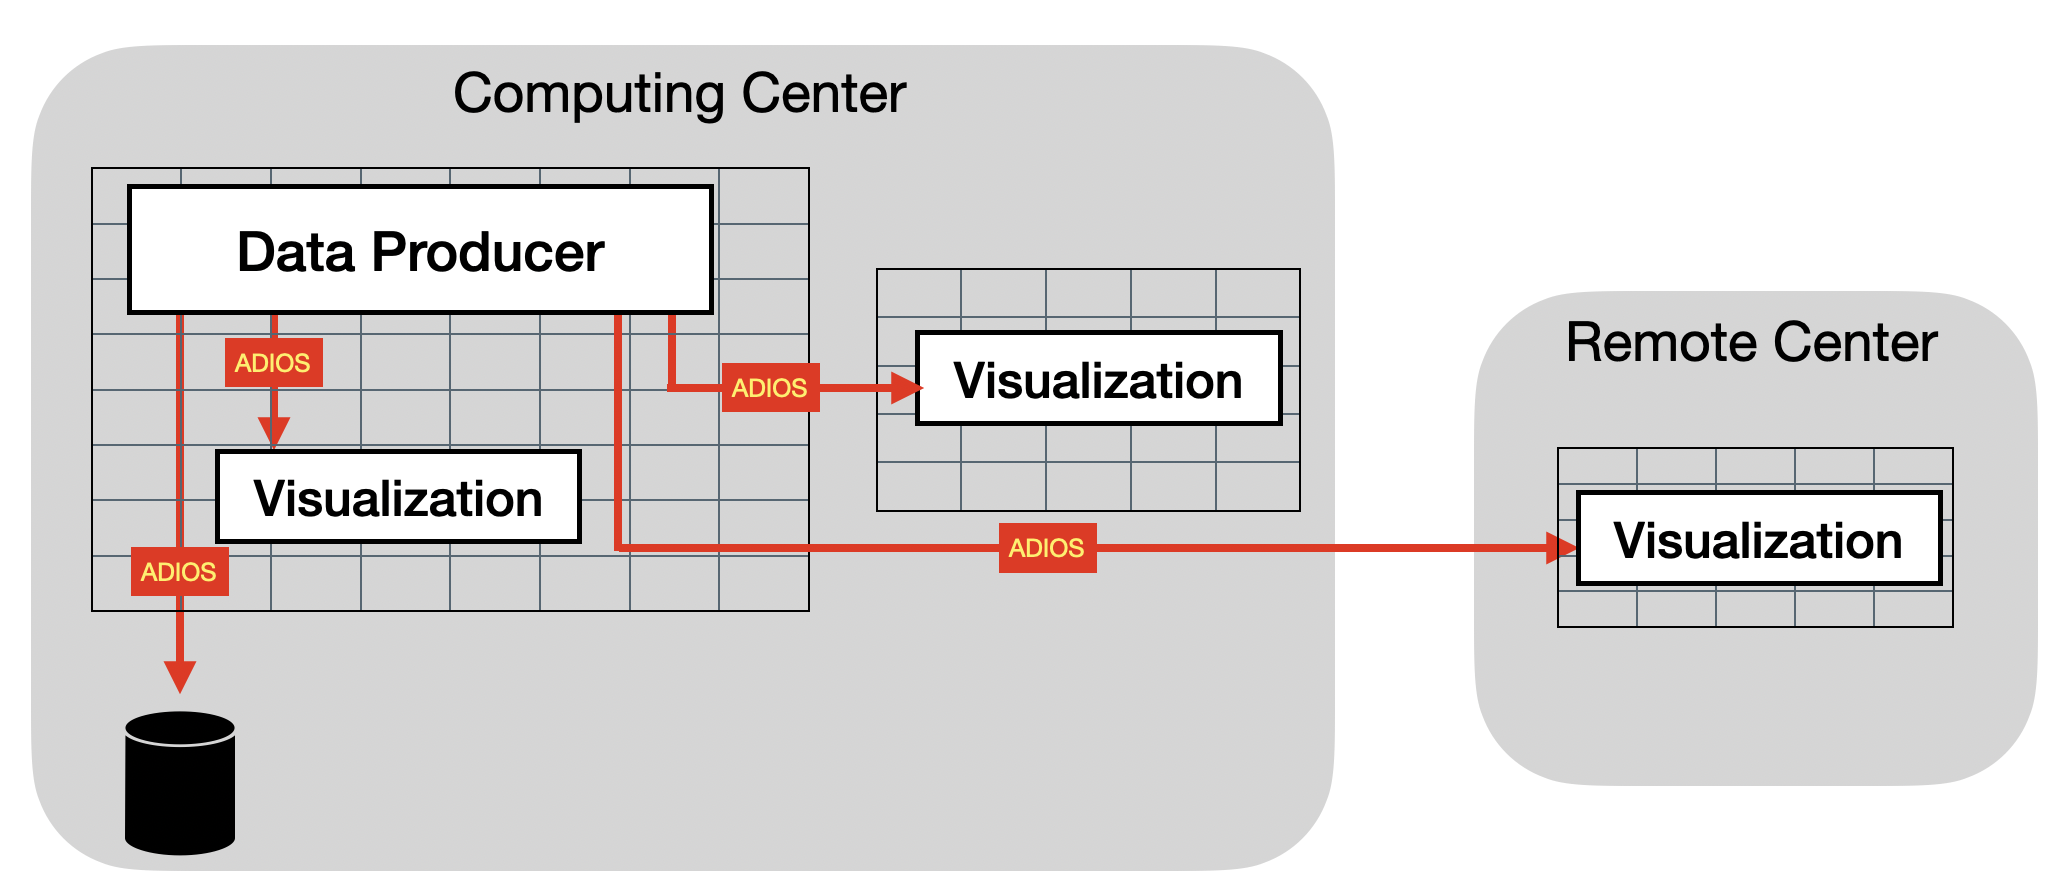
\includegraphics[width=4in]{figures/ADIOS}
    \caption{Examples of ADIOS usage. In this example, the producer can write data to disk, to a visualization process sharing the same resource as the simulation, to a separate set of nodes, or across the network to a remote computing center.}
    \label{ch10:fig:adios_design}
\end{figure}


In terms of the taxonomy described in Section~\ref{intro:taxonomy} of Chapter~\ref{chapter:intro}, ADIOS can be classified in the following ways. \emph{Integration type}: Apart from the usage of the ADIOS API for I/O, no additional instrumentation is needed by the application. \emph{Proximity}: The visualization can run on the same or different computing resources. \emph{Access}: The visualization can directly access memory in the simulation, or it can be copied to a memory buffer on the same or on different computing resources. \emph{Division of Execution}: Synchronous or asynchronous are both possible, providing support for both time and space division.  \emph{Operation Controls}: Human in the loop is possible using both synchronous (blocking) or asynchronous (non-blocking) modes.


The ADIOS framework design was based on the goal to provide an I/O abstraction for parallel and distributed applications that expresses \emph{what} data is produced for output and \emph{when} that data is ready for output, or what data an application wants to read and when\cite{liu2014hello, Logan2020, osti_1468120}.
This is achieved in ADIOS through the use of different types of I/O \emph{engines}. When an application writes a set of data, it uses the appropriate engine (e.g., File engine, In situ engine, etc) to do the actual data movement. Similarly for a reader, it uses the appropriate Engine to request the data that it needs. For flexibility, the types of engine used by producer and consumer can be specified in a configuration file for runtime selection.
In this way, applications that either read or write data need only select the appropriate output engine, and do not need to be concerned with the implementation details needed to achieve scalable performance.


%ADIOS was designed with the observation that, from an application point of view, there is not much difference between writing and reading data from storage and coupling independent application codes together.
%The main goal of the ADIOS framework design is to provide an I/O abstraction for parallel and distributed applications, that expresses \emph{what} data is produced for output and \emph{when} that data is ready for output, or what data an application wants to read and when.
%Crucially, the concept of permanent storage or a connected application, i.e., the target of the output or the source of the input, is omitted from the abstraction.
%The I/O \emph{strategy} is dependent on what the input sources and output targets are, and is implemented by a designated ADIOS \emph{Engine}.
%Therefore, an application can use ADIOS to produce an output data stream without concerning itself with where the data goes, and then choose the proper engine at runtime to store data on disk or to stream it to a consumer application. 

The separation of concerns, namely that an application only need to be concerned about the data production and consumption but not how the data should be delivered, allows for creating optimized ADIOS engines that all can work with the same application code.
Using the ADIOS interface makes application I/O \emph{scalable}, a primary goal of the ADIOS framework, which is designed to work well on the largest supercomputers. ADIOS regularly runs on the largest supercomputers in the world for applications that consume and produce multiple petabytes of data during the course of a simulation run.

%There are applications, like Specfem3d\_globe\cite{specfem3d}, PIConGPU\cite{picongpu} and XGC\cite{xgc}, that regularly produce and consume petabytes of data on the leadership computing facilities around the world using ADIOS for storage I/O. 

In this chapter we describe details of the ADIOS framework and how it can be used for in situ visualization. In Section~\ref{sec:adios} we describe the I/O abstractions used by ADIOS and how applications and visualization codes can use them. Section~\ref{sec:adios:engine} provides a description of the engines provided by ADIOS and how they handle the movement of data. Advanced features in ADIOS are described in Section~\ref{sec:adios:advanced}, followed by a  discussion on the relative strengths of each engine and coding examples in Sections~\ref{sec:adios:discussion} and~\ref{sec:adios:code}. In Section~\ref{sec:examples} we describe the use of ADIOS for in situ visualization with application partners, followed by some concluding remarks in Section~\ref{sec:conclusion}.

%In this chapter, we focus on other capabilities borne from this I/O abstraction. Since the application output code only defines what the output data is and when it is ready for output but does not encode anything about how the output is performed, the output data can move to different targets depending on the engine that connects the application to the target. It can be used for strong coupling of simulation codes, for in situ visualization running on a separate computing cluster, and for streaming experimental data between Asia and the United States.


\section{ADIOS I/O Abstraction}
\label{sec:adios}

A parallel application that produces data uses ADIOS to define \emph{variables} ($n$-dimensional distributed arrays of a particular type) and \emph{attributes} (labels associated with individual variables or the entire output data set).
It also specifies when the data is available for output. The output is organized around output \emph{Steps}, instead of individual variables.
A Step includes all the variables and attributes that are to be sent to the target at once.
There is nothing in the ADIOS interface that prescribes how to handle the data (e.g. data aggregation among the processes, targeting a single file or one file per process, handling multiple readers, and handling the disappearance of a potential reader).
These belong to the \emph{IO strategy} and are implemented in various ways by different Engines.
The user can control the behavior of the application by choosing a specific engine, and parameterizing it with available options. 

Similarly, a reading application only declares what data it wants to retrieve from a source, each process of the parallel application declaring what it needs, and when it expects the data to be in its memory.
The input is also organized around Steps, not individual variables. The semantics of the ADIOS API  ensure that a reader never gets into an inconsistent state where portion of the data of some variables belong to a certain step, and other portion to another step.

Analysis and visualization are typically data-hungry operations~\cite{Childs2010}. This makes scalable access to data key. In an in situ environment, the ability to maintain clear boundaries between simulation and analysis tasks can promote fault tolerance, interoperability, programmability and maintainability.  


The flexibility of the data movement abstractions provided by ADIOS makes it easy to integrate with analysis and visualization applications. The ``file-like'' API provided by ADIOS allows seamless reads from disk, from memory, or streaming over the network.
Likewise, on the write side, outputs produced by analysis and visualization applications can be written to disk, or shared with other applications through memory or streamed over the network. The abstraction used by ADIOS makes it easy to move data as it does something that the application is already doing, namely, reading and writing from files.

The abstraction provides the same access to data regardless of where the data are located, be it disk, memory or streaming. 
As examples, the  VisIt~\cite{HPV:VisIt} and ParaView~\cite{paraview} visualization tools have support for reading data from ADIOS in this manner.
Both tools provide access to ADIOS data using a data reader plugin.
The plugin reads the ADIOS data and creates mesh-based data that can be visualized by the VisIt and ParaView tools.
An example of VisIt visualizing streaming data is described in Section~\ref{sec:jaxa}.

When visualization is used in an in situ environment, the ability to have clear boundaries between the simulation and analysis and visualization, and rely on a middleware layer for the sharing and exchange of data is valuable in a number of ways. 
(1) It makes it much easier to reconfigure components in a workflow based on the needs of the scientific campaign. (2) Fault tolerance is increased because the simulation can be separated from the visualization. (3) The mechanism for sharing data between producer and consumer can more easily be modified, changed or replaced.

In the remainder of this section we describe ADIOS in more detail. In Section~\ref{sec:adios:engine} and~\ref{sec:adios:advanced} we describe the ADIOS engines used to move data and some advanced topics on reduction and data interpretation.
In Section~\ref{sec:adios:discussion} we discuss the characteristics of these engines and how they relate to visualization and analysis needs and costs. Finally, in Section~\ref{sec:adios:code} we show some code examples of how ADIOS is used for both data producers and data consumers.

\subsection{ADIOS Engines}
\label{sec:adios:engine}

The mechanism in ADIOS for moving data is called an \emph{engine}.
An engine is tasked with executing the I/O heavy operations associated with the movement of data. 
Each engine supports a unified interface that allows data producers to \emph{put} data, and data consumers to \emph{get} data. The details of moving the data between source and destination are left to particular implementation details of each engine.
ADIOS provides a number of engines, which are described below.

\subsubsection{File-based Engines}
ADIOS provides two types of engines for performing parallel IO of data to disk storage. 

\paragraph{\textbf{BPFile Engine}}
The BPFile engine is the default engine for storage.
The output file target is a directory, which contains both metadata and  data files. The number of files is tailored to the capability of the file system, not to the number of writers or readers, which ensures scalable I/O performance. The steps stored in a single file target, can be read by other applications step-by-step simultaneously. Therefore, this engine can be used for in situ processing through the file system.

\paragraph{\textbf{HDF5 Engine}}
This engine can be used to write and read HDF5 formatted files. It uses the Parallel HDF5 library, so it provides only a compatibility layer to process HDF5 files in an ADIOS application workflow and is only as scalable as the HDF5 library itself. Streaming access to data is not currently available, but will be available once it is supported by HDF5.
 
\subsubsection{Data Staging Engines}
Data staging is a generic concept in ADIOS for providing concurrent access to data to one or more consumers through memory or streamed over the network. It can map onto both time and space division of the taxonomy in Chapter~\ref{chapter:intro}. Data staging engines are typically used for doing in situ analysis and visualization and code coupling. With staging engines, the data producer will write the data using the ADIOS API. The data are then available to be read by the consumers using the ADIOS API. Each staging engine has the ability to move the data in different ways, which are described below.

\paragraph{\textbf{Scalable Staging Transport (SST)}}
The most versatile and flexible staging engine uses either RDMA, TCP, UDP, or shared memory to move data from a producer (parallel application) to other consumers (multiple independent parallel applications). Consumers can come and go dynamically without affecting the producer. The output step is buffered in the producer's memory, and readers pull out portions of the buffered data with RDMA operations or communicate with a thread in the producer to receive it via TCP. The requirement of all engines to always provide a consistent view of a step to a reader may result in blocking the producer from progressing if the consumer is slower than the producer. The SST writer engine aggregates metadata for every step, and shares it with all readers. Readers then issue remote reading operations based on the I/O pattern in metadata. This allows the I/O pattern to vary over time. SST also allows readers to disconnect and reconnect while writers keep writing.
To address different application requirements, the SST buffering policy can be configured at run-time. This includes keeping only the most recent step, buffering a fixed window of consecutive steps, or blocking until the step is consumed. In cases where strong coupling is required between applications, the buffer limit can be set to $1$, which ensures that every step is consumed by the reader before the producer moves to the next data step.
For use cases like interactive visualization, buffering only the latest step is useful since the user typically does not want to block the simulation while a particular time step is explored.
While SST aims to provide the flexibility for addressing various application requirements, the fact that it manages metadata for every single step may be overkill for uses cases where the metadata does not change frequently, or at all.
 
\paragraph{\textbf{Insitu-MPI}}
This engine focuses on the speed of data movement for use cases where the metadata is constant across the workflow and a single metadata aggregation at the first data step will suffice. After this first step, each writer and reader knows the exact I/O pattern and direct communication is performed using asynchronous send and receive operations using an MPI  communicator. Since it uses MPI, the producer and consumer applications must be launched within a single mpiexec command using the Multiple Program Multiple Data (MPMD) mode. The engine directly sends the application data to the consumer, hence, the producer is synchronized to the consumer at every step to avoid modifying the data before it is received. 
For very large applications with constant I/O patterns, the Insitu-MPI engine can provide CPU savings for metadata management. However, since it must be launched in MPMD mode under MPI, the flexibility of readers dynamically join or leave is not supported at run-time.


\paragraph{\textbf{Staging for Strong Coupling (SSC)}}
The SSC engine is also designed for applications that have constant metadata over time. Similar to the Insitu-MPI engine, the SSC engine aggregates metadata once on the first time step. The main differences between SSC and Insitu-MPI are that SSC uses one-sided MPI communication and that the producer output is buffered.
The one sided MPI paradigm does not require the send and receive calls to be paired. Instead, it allows direct access to remote memory of another process. The buffering of application data, on the other hand, enables the producer to continue with the computation while the data is transferred to the consumer. 
In very large scale coupling use cases this approach saves the overhead of one side waiting for the other side to complete the send and receive pairs, and makes it possible for applications to very quickly, and frequently exchange data. 


\paragraph{\textbf{DataMan}}
This engine focuses on providing good bandwidth over wide-area-networks (WAN. It uses the publish and subscribe communication mechanism of the ZeroMQ library and has been optimized specifically for long-distance low-latency data movement. Unlike other staging engines, such as SSC described above, DataMan does not guarantee that every data step is transferred. Instead, the subscriber is designed to read only the latest data steps, while ignoring the previous steps. This saves the two-way communications for checking step completion, which usually means several hundred milliseconds in inter-continental data transfers. Because of this, the data transfer latency is greatly reduced and can support near-real-time analysis better than other engines over the WAN.

\subsection{Advanced Data Management Services}
\label{sec:adios:advanced}
ADIOS has a number of internal and external supports for advanced management of data. These include data compression, and schemas for providing additional information about ADIOS data to help downstream processing applications, such as analysis and visualization to properly interpret the raw data.

\subsubsection{Data Compression}
ADIOS supports operators as a mechanism for performing calculations on the data before it is written by an engine.
A general purpose operator, called a Callback provides the user with the ability to perform arbitrary calculations and manipulations to the data inside the engine. Data compression is provided in ADIOS using this mechanism. It provides support for a number of different lossless and lossy compression methods, which are described below.

In the classical workflow for high-performance scientific simulations, the entire data set is written to storage after generation.
This will no longer be viable at the exascale, simply because the amount of data will swamp the filesystem.
To accelerate scientific discovery, we must prioritize information over data.
It will be vital to take advantage of a priori user information to prioritize the most useful data so that I/O can be completed under standard HPC time constraints.
(For example, on Summit, jobs are limited to 24 hours.)
One solution is data compression.
ADIOS supports storing or transporting data in compressed form to reduce the I/O cost while preserving key information, which in turns speed up simulations or in situ data analysis and visualization~\cite{chenunderstanding}.
Enabling compression requires minimal development effort from users.
Simply specifying an operator for each variable enables ADIOS to automatically compress or decompress at the point of data publication or subscription.
Lossless compressors such as BZip2~\cite{seward1996bzip2} preserve every bit of the data, but compression ratios observed in practice are minimal.
Lossy compressors such as MGARD~\cite{ ainsworth2018multilevel,ainsworth2019multilevel2,ainsworth2019multilevel}, SZ~\cite{di2016fast, liang2018efficient,tao2017significantly}, and ZFP~\cite{lindstrom2014fixed} provide much higher compression ratios (usually more than an order of magnitude than lossless), but information is lost.
However, most lossy compressors allow control of the loss through parameters, which can be easily set in ADIOS.
Also, as derived quantities in data are particular important for scientific discovery, one of the compressors supported by ADIOS, MGARD, can consider one or more relevant quantities of interest and reduce the data so as to preserve these quantities.
Furthermore, ADIOS supports the meta-compressor Blosc which provides further lossless compressors (Zstd, Snappy, BloscLZ, LZ4HC) as well as shuffle pre-conditioners.
In GPU-centric applications, using ADIOS with Blosc's threaded-chunked compressor variants regularly trades unutilized CPU-cycles for I/O speedup~\cite{Huebl2017}.


\subsubsection{Schemas}
Schemas provide the ability to annotate the semantics of the array-based layout of data in ADIOS.
These provide the meaning of each data array, and the relationship between groups of arrays in an ADIOS file or stream. 
This capability makes it easier for tools using ADIOS to be used together in, for example, a complex scientific workflow.
Two examples of such schemas are described below.

%% I guess there is no subsubsubsection...
%\subsubsubsection{ADIS Visualization Schema}
\paragraph{\textbf{ADIS Visualization Schema}}
%As simulations become more ambitious, the cost of running an irrelevant or buggy job increases proportionally.
%Real-time graphical analysis of a simulation is a form of quality control, but to our knowledge, software tools which facilitate this have not been developed.
%The SST staging engine of ADIOS, along with the high-performance computer graphics library VTK-m can be glued together with the newly written ADIS library, so that real-time graphical analysis of a simulation can be performed.
%For example, using ADIS, we can visualize a timestep in an ODE or PDE solver \emph{as it is being computed}.
%This is an extremely useful quality control step, as in many contexts, timesteps occupy so much memory that they must be discarded, with only the final timestep being visualized.
%This is a very dangerous numerical simulation, with quality control only being done at the final state.
%The three technologies of ADIS, ADIOS, and VTK-m allows complete decoupling between numerical simulation and graphical quality control.
%Note that some hardware resources must be devoted to graphical analysis, but Amdahl's law suggests that the final performance cost will not be too great.


The Adaptable Data Interface for Services (ADIS) is a schema for describing mesh-based data that are used by visualisation tools. ADIS uses a JavaScript Object Notation (JSON) formatted strings to describe the content of ADIOS data. For example, for ADIOS data arrays representing field data on a uniform grid, the ADIS schema will specify that there is a uniform mesh of a given size, and the names of the arrays in the ADIOS stream for each field and the association on the mesh (e.g., zone centered, point centered, etc).
For more complex mesh types, like unstructured grids, ADIS specifies the names of the arrays for specifying the relevant mesh structures (e.g., point  coordinate values, cell information, etc).

ADIS also supports the creation of data sets from ADIOS in the VTK-m~\cite{moreland2016} format. Given a schema, and an ADIOS file/stream, ADIS will read data from ADIOS and construct the appropriate VTK-m data object.

\paragraph{\textbf{openPMD Schema}}

The Open Standard for Particle-Mesh Data Files (openPMD) is a schema for describing mesh- and particle-based data.
% standardized metadata to exchange, archive, reproduce, and visualize generated data products and automate scientific data workflows as a critical aspect in productive I/O
Its primary focus is the exchange, archival and replicability of scientific data via a minimal set of conventions and meta information.
The schema is defined in the so-called "base standard" and "extensions".
The former is agnostic of the data's scientific domain and can be automatically verified/parsed, visualized, scaled and dimensionally analyzed (describing units and quantities).
The base standard also provides means to document authorship, hardware and software environments towards reproducible research.
Based on this, standardized meta-information in openPMD schema "extensions" add further meaning for domain-scientists, e.g. by documenting algorithms and methods that generated a data set.

Contrary to visualization-focused and domain-specific schemas, openPMD is a notion for \textit{scientifically self-describing} data in general, providing a unified description for data in scientific workflows from source, over processing, analysis and visualization to archival in (open) data repositories.
% a unified description for post-processing, visualization and analysis.
% This standard tries to bridge the gap between the common "blob of data" and the algorithms, methods and/or schemes that created these.
openPMD is widely adopted in plasma-physics, particle-accelerator physics, photon-science, among others.\footnote{Curated list available at \url{https://github.com/openPMD/openPMD-projects}}
% Data analysis and Vis: VisIt, yt, domain-specific, ...
% converters: GPT, VTK-files, ...

The schema can be added to data described via hierarchical, self-describing (portable) data formats.
Open implementations are available in C++, Python and Fortran and currently range from MPI-parallel ADIOS1, ADIOS2 and HDF5 library backends to serial JSON files.
The openPMD schema is versioned, citable and developed on GitHub.
Its release is version 1.1.0 and data files using the schema are forward-updatable via lightweight meta-data transformations~\cite{HueblopenPMD}.
% GitHub-centric community contribution process


\subsection{Discussion}
\label{sec:adios:discussion}

\begin{figure}[t]
\sidecaption
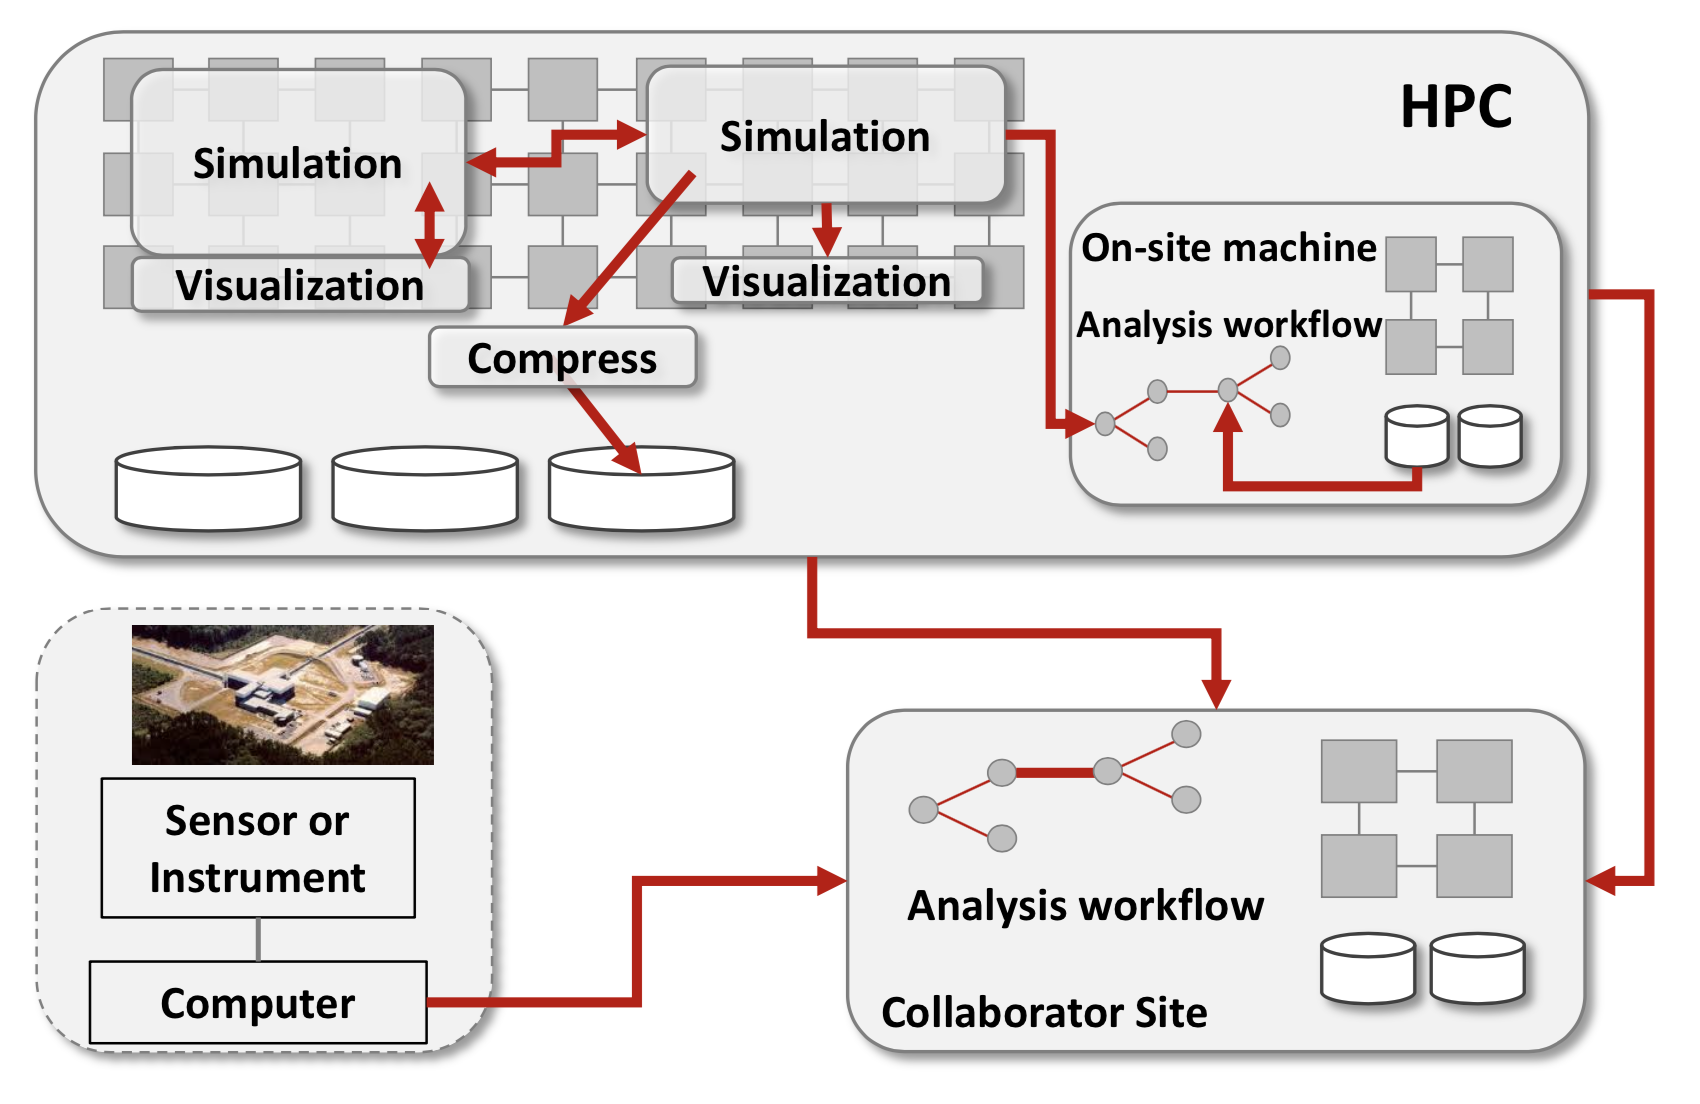
\includegraphics[width=1\linewidth]{figures/ADIOS_workflow.png}
\caption{Example workflow using ADIOS for simulation coupling, in situ visualization, in transit visualization, and streaming of both simulation and experimental data over the WAN to a remote site for analysis.}
\label{fig:example_workflow}
\end{figure}

The number of engines available in ADIOS provides a large amount of flexibility when selecting a configuration. Further, multiple executables can be connected using the read/write API of an ADIOS engine to support a range of different types of workflows. The example workflow in Figure~\ref{fig:example_workflow} shows ADIOS (indicated with red arrows) being used as the data movement mechanism for a number of tasks. It is used to couple two simulations, in situ visualization on the HPC resource, in transit visualization on a cluster in the HPC center, and transfer data over the WAN to remote site for analysis. Additionally, data from a sensor/experiment is streamed over the WAN for analysis that uses simulation results.

When designing a visualization workflow, the choice of engine for each component is dependent on a number of factors. Broadly speaking these classes of visualization are post hoc, in situ (time division), and in transit (space division). Post hoc visualization is the traditional mode of visualization where the data are read from disk. As discussed in Chapter~\ref{chapter:intro}, in situ visualization, while a broadly defined term, is for simplicity, the case where the visualization and simulation use the same set of resources. In transit visualization uses two distinct sets of resources, one dedicated to the simulation and the other dedicated to the visualization. The network is used to transfer data between the two sets of resources. Below, we discuss these three modes from the ADIOS and visualization perspectives and the impact of choices made have on visualization functionality and performance.

\subsubsection{ADIOS Perspective}
From an ADIOS perspective, the following three characteristics are important: (1) data access and movement, (2) fault tolerance, and (3) programmability.

\paragraph{\textbf{Data Access and Movement}}
Data access is defined as how much of the total spatio-temporal data are available, as the temporal range of data that are available. Data movement is the amount of data that must be moved from producer to consumer.
\begin{itemize}
    \item \textbf{Post hoc:} Has access to all the spatio-temporal data that have been saved. However, the data movement cost is highest, and may restrict the amount of data available.
    \item \textbf{In situ / time division:} Has the highest access and lowest movement costs for spatio-temporal data as resources are shared with the producer. Access to multiple temporal steps requires additional on-node resources.
    \item \textbf{In transit / space difision:} Data access is configurable based on needs. The dedicated resource can be sized to control the amount of spatio-temporal access, as well as temporal range. Since data movement occurs over the internal network, it is much faster than I/O.
\end{itemize}

\paragraph{\textbf{Fault Tolerance}}
Fault tolerance describes the relative robustness of the system with respect to faults occurring in either the producer or the consumer.
\begin{itemize}
    \item \textbf{Post hoc:} The consumer is independent from the data producer, so fault tolerance is very high.
    \item \textbf{In situ / time division:} Because resources are shared, the producer and consumer can impact each other. This includes faults, memory corruption, memory usage, etc.
    \item \textbf{In transit / space division:} Like post hoc, the consumer is independent from the data producer. Faults occurring on the dedicated nodes will not impact the producer.
\end{itemize}


\paragraph{\textbf{Programmability}}
Programmability describes the relative ease and flexibility of connecting a simulation with visualization. This includes composing a workflow, connecting components in a workflow, and modifying the underlying data movement mechanism. Since all three classes of visualization use the same abstraction, the programmability is improved by simply  changing the engine used.

Table~\ref{table:adios_char} provides a visual representation of the relative strengths of each ADIOS engine with respect the characteristics described above. A score for each engine is assigned 
based on how well the engine performs with respect to each characteristic described above. A $``+"$ signifies a favorable evaluation, $``-"$ a less favorable evaluation, and $``0"$ for in between.


\begin{table}[b]
\centering
\caption{Characterization of each ADIOS engine}
\label{table:adios_char}
\renewcommand{\arraystretch}{1.75}
\setlength{\tabcolsep}{2.6pt}
\begin{tabular}{p{1mm}c|cccccc}
\hline
 & \cellcolor[HTML]{EFEFEF} & \multicolumn{6}{c}{\cellcolor[HTML]{EFEFEF}\textbf{Engine Type}} \\
 & \multicolumn{1}{c|}{\cellcolor[HTML]{EFEFEF}\textbf{ADIOS Characteristics}} & \cellcolor[HTML]{EFEFEF}\textbf{BPFile} & \cellcolor[HTML]{EFEFEF}\textbf{HDF5} & \cellcolor[HTML]{EFEFEF}\textbf{SST} & \cellcolor[HTML]{EFEFEF}\textbf{Insitu-MPI} & \cellcolor[HTML]{EFEFEF}\textbf{SSC} & \cellcolor[HTML]{EFEFEF}\textbf{DataMan} \\ \hline
 & \textit{Spatial Access} & + & + & 0 & 0 & 0 & 0 \\
 & \textit{Temporal Fidelity} & - & - & + & + & + & 0 \\
 & \textit{Temporal Range} & + & + & 0 & 0 & 0 & 0 \\
\multirow{-4}{*}{\rotatebox[origin=c]{90}{\pbox{23mm}{\textbf{Data Access \& Data Movement}}}} & \textit{Movement} & - & - & 0 & 0 & + & 0 \\
\hline
 & \multicolumn{1}{c|}{\cellcolor[HTML]{EFEFEF}\textbf{Fault Tolerance}} & + & + & + & + & 0 & + \\
\hline
 & \multicolumn{1}{c|}{\cellcolor[HTML]{EFEFEF}\textbf{Programability}} & + & 0 & + & + & + & + \\ \hline
\end{tabular}
\end{table}

%\begin{table}[b]
%\centering
%\caption{Characterization of each ADIOS engine }
%\label{table:adios_char}
%\renewcommand{\arraystretch}{1.5}
%\setlength{\tabcolsep}{2.6pt}
%\begin{tabular}{c|cccccc}
%\hline
%\rowcolor[HTML]{EFEFEF} 
%\multicolumn{1}{l|}{\cellcolor[HTML]{EFEFEF}} & \multicolumn{6}{c}{\cellcolor[HTML]{EFEFEF}\textbf{Engine %Type}} \\
%\rowcolor[HTML]{EFEFEF} 
%\textbf{ADIOS Characteristics} & \textbf{BPFile} & \textbf{HDF5} & \textbf{SST} & \textbf{Insitu-MPI} & %\textbf{SSC} & \textbf{DataMan} \\ \hline
%\cellcolor[HTML]{EFEFEF}\begin{tabular}[c]{@{}c@{}}\textbf{Data Access/Movement}\\\emph{(Spatial, %Temporal,}\\\emph{Temporal Range, Movement)}\end{tabular} & - - + - & - - + - & 0 0 0 0 & + + - + & + + - + & %0 0 0 - \\
%\cellcolor[HTML]{EFEFEF}\textbf{Fault Tolerance} & + & + & + & - & - & + \\
%\cellcolor[HTML]{EFEFEF}\textbf{Programmability} & + & + & + & + & + & + \\ \hline
%\end{tabular}
%\end{table}

\subsubsection{Visualization Perspective}
From a visualization perspective, a different set of characteristics are important (see for example, ~\cite{Kress-isav15}).
We discuss the following characteristics below: (1) scalability and resource requirements, (2) interactivity, (3) fault tolerance, and (4) programmability.

\paragraph{\textbf{Scalability and Resource Requirements}}
Scalability is defined as how efficiently the visualization task can use the allocated resources.
Resource requirements is defined as the need for additional resources beyond that of the simulation.
\begin{itemize}
    \item \textbf{Post hoc:} Has the flexibility to allocate resources suitable for the required tasks, however I/O can slow for large data.
    \item \textbf{In situ / time division:} Since the visualization must run at the scale of the visualization, the performance will depend on the operation. Communication heavy algorithms could suffer poor performance at larger scales.
    \item \textbf{In transit / space division:} Has the flexibility to allocate resources suitable for the required tasks. Since I/O is avoided, access to data can be much faster.
\end{itemize}

\paragraph{\textbf{Interactivity}}
Interactivity is defined as the ability for a user to interact with the data, select regions of interest, and plot the data to extract understanding.
\begin{itemize}
    \item \textbf{Post hoc:} Because visualization is independent from the simulation, full interactivity is possible with all data available.
    \item \textbf{In situ / time division:} Visualization has full access to all of the data that are available on the simulation resources. Due to limited available resources, the temporal range of data could be limited. If the data are shared, the simulation could be blocked while visualization occurs.
    \item \textbf{In transit / space division:} Visualization has full access to all of the spatio-temporal data that are moved to the dedicated resources. Because the data are not shared with the simulation, blocking can be avoided.
\end{itemize}


\paragraph{\textbf{Fault Tolerance}}
As above, fault tolerance refers to the robustness of the visualization to avoid impacting the simulation.
\begin{itemize}
    \item \textbf{Post hoc:} Visualization is independent from the simulation, so fault tolerance is very high.
    \item \textbf{In situ / time division:} Because resources are shared, it is possible for the visualization task to negatively impact the simulation.
    \item \textbf{In transit / space division:} Like post hoc, the visualization is independent from the simulation. Errors occurring on the dedicated nodes will not impact the simulation.
\end{itemize}

\paragraph{\textbf{Programmability}}
As above, programmability describes the ease of using visualization tools with simulation data in a variety of configurations. This includes performing visualization tasks within a workflow, connecting analysis and visualization tasks together, and the ability to access data from different sources.
 Since all three classes of visualization use the same abstraction, the programmability is improved by simply  changing the engine used.

Table~\ref{table:visualizationImportantChar} provides a visual representation of the relative strengths of each ADIOS engine with respect the important visualization characteristics described above. As above, a $``+"$ signifies a favorable evaluation, $``-"$ a less favorable evaluation, and $``0"$ for in between.
\begin{table}[htb]
\centering
\renewcommand{\arraystretch}{1.5}
\setlength{\tabcolsep}{2.3pt}
\caption{Characterization of each ADIOS engine for visualization}
\label{table:visualizationImportantChar}
\begin{tabular}{p{0.1mm}c|cccccc}
\hline
\multicolumn{1}{l}{} & \multicolumn{1}{l|}{\cellcolor[HTML]{EFEFEF}} & \multicolumn{6}{c}{\cellcolor[HTML]{EFEFEF}\textbf{Engine Type}} \\
\multicolumn{1}{l}{} & \cellcolor[HTML]{EFEFEF}\textbf{Visualization Characteristics} & \cellcolor[HTML]{EFEFEF}\textbf{BPFile} & \cellcolor[HTML]{EFEFEF}\textbf{HDF5} & \cellcolor[HTML]{EFEFEF}\textbf{SST} & \cellcolor[HTML]{EFEFEF}\textbf{Insitu-MPI} & \cellcolor[HTML]{EFEFEF}\textbf{SSC} & \cellcolor[HTML]{EFEFEF}\textbf{DataMan} \\ \hline
 & \textit{Data} & - & - & + & + & + & - \\
 & \textit{Communication} & + & + & + & - & - & + \\
\multirow{-3}{*}{\rotatebox[origin=c]{90}{\textbf{Scalability}}} & \textit{Resource} & + & + & - & + & + & - \\
\hline
 & \textit{Spatial} & - & - & 0 & + & + & 0 \\
 & \textit{Temporal} & - & - & 0 & + & + & 0 \\
 & \textit{Temporal Range} & + & + & 0 & - & - & 0 \\
\multirow{-4}{*}{\rotatebox[origin=c]{90}{\textbf{Interactivity}}} & \textit{Block Simulation} & + & + & + & - & - & + \\
\hline
\multicolumn{1}{l}{} & \cellcolor[HTML]{EFEFEF}\textbf{Fault Tolerance} & + & + & + & + & 0 & + \\
\hline
\multicolumn{1}{l}{} & \cellcolor[HTML]{EFEFEF}\textbf{Programability} & + & 0 & + & + & + & + \\ \hline
\end{tabular}
\end{table}


%\begin{table}[h]
%\centering
%\label{table:}
%\renewcommand{\arraystretch}{1.5}
%\setlength{\tabcolsep}{2.3pt}
%\begin{tabular}{c|cccccc}
%\hline
%\rowcolor[HTML]{EFEFEF} 
%\multicolumn{1}{l|}{\cellcolor[HTML]{EFEFEF}} & %\multicolumn{6}{c}{\cellcolor[HTML]{EFEFEF}\textbf{Engine Type}} \\
%\rowcolor[HTML]{EFEFEF} 
%\textbf{Visualization Characteristics} & %\multicolumn{1}{c}{\cellcolor[HTML]{EFEFEF}\textbf{BPFile}} & %\multicolumn{1}{c}{\cellcolor[HTML]{EFEFEF}\textbf{HDF5}} & %\multicolumn{1}{c}{\cellcolor[HTML]{EFEFEF}\textbf{SST}} & %\multicolumn{1}{c}{\cellcolor[HTML]{EFEFEF}\textbf{Insitu-MPI}} & %\multicolumn{1}{c}{\cellcolor[HTML]{EFEFEF}\textbf{SSC}} & %\multicolumn{1}{c}{\cellcolor[HTML]{EFEFEF}\textbf{DataMan}} \\ \hline
%\cellcolor[HTML]{EFEFEF}\begin{tabular}[c]{@{}c@{}}\textbf{Scalability}\\ \emph{(Data, %Communication, Resource)}\end{tabular} & - + + & - + + & + + - & + - + & + - + & - + - %\\
%\cellcolor[HTML]{EFEFEF}\begin{tabular}[c]{@{}c@{}}\textbf{Interactivity}\\\emph{(Spati%al, Temporal,}\\\emph{Temporal Range, Block Sim.)}\end{tabular} & - - + + & - - + + & 0 %0 0 + & + + - - & + + - -& 0 0 0 + \\
%\cellcolor[HTML]{EFEFEF}\textbf{Fault Tolerance} & + & + & + & - & - & + \\
%\cellcolor[HTML]{EFEFEF}\textbf{Programmability} & + & + & + & + & + & + \\ \hline
%\end{tabular}
%\end{table}



\subsubsection{In Situ Data Placement and the Associated Performance Implications}
\label{sec:implications}
Placement (in-line, in-transit, hybrid methods) is an important aspect to consider when planning for the use of in situ techniques. Performance can vary drastically depending on what analysis operations are used, how often they are performed, and at what scale they are performed. This performance difference is due primarily to the scaling characteristics of the analysis algorithms in relation to that of the underlying simulation, and can have a large effect on the overall cost of a simulation plus its visualization and analysis components. 

In a work by Kress et al.~\cite{kress2019comparing} they look specifically at the cost of performing isocontours and ray tracing with parallel compositing both in-line and in-transit, and observe large cost variations based on placement as the simulation was scaled. Their work found that as the simulation was scaled to 16K cores, that visualization algorithms suffered large slowdowns in-line. However, if the data was transferred from the simulation over the network to a set of dedicated visualization nodes that the visualization routines completed much faster. They bring up a couple of general guidelines in that work: (1) if fastest time to solution is your goal at scale, moving the data and performing the visualization in-transit is the best solution; (2) if the lowest total combined cost of the simulation and visualization routines are the overall goal, the solution becomes more complicated. In general though, as the simulation scales if the visualization routines do not scale as well, moving the visualization routine to a smaller in-transit allocation is the best choice. However, careful consideration has to be given to how large of an in-transit allocation to reserve, and how often the visualization should be performed. A follow on work~\cite{kress2020Cost} develops a cost model to evaluate the use of in situ methods at scale.


\subsection{Code Examples}
\label{sec:adios:code}
This section contains examples using ADIOS to read and write data.
The first example, shown in Listing ~\ref{code:writeExampleFile}, illustrates how a simulation code would write output data to disk using the BPFile engine.
The engine type is specified in line~\ref{code:writeExampleFile:engineType}.

\lstset{language=C++,
        basicstyle=\ttfamily\scriptsize,
        showstringspaces=false,
        numbers=left,
        keywordstyle=\color{blue}\ttfamily,
        stringstyle=\color{red}\ttfamily,
        commentstyle=\color{magenta}\ttfamily,
        morecomment=[l][\color{magenta}]{\#},
        escapechar=|
}

\begin{minipage}{\linewidth}
\begin{lstlisting}[frame=single,label={cxxAPI},caption={Example of simulation writing outputs to a file.}, label=code:writeExampleFile]
adios2::ADIOS adios(MPI_COMM_WORLD); |\label{code:writeExampleFile:configType}|
// Declare named IO process
adios2::IO io = adios.DeclareIO("output");

// Declare output type and size.
adios2::Variable<double> var = 
  io.DefineVariable<double>("var", globalDims, offset, localDims);
                                

// Set engine output to BPFile
io.SetEngine("BPFile"); |\label{code:writeExampleFile:engineType}|
adios2::Engine engine = io.Open("output.bp", adios2::Mode::Write);

// Run Simulation
for(...)
{
   double *data = Simulation();
   
   engine.BeginStep();
   engine.Put(var, data);
   engine.EndStep();
}
engine.Close();
\end{lstlisting}
\end{minipage}

Listing~\ref{code:readExampleFile} shows a program that reads data from the output file and performs visualization on the data.

\begin{minipage}{\linewidth}
\begin{lstlisting}[frame=single,label={cxxAPI},caption={Example of a visualization  program reading data from a file}, label=code:readExampleFile]
adios2::ADIOS adios(MPI_COMM_WORLD); |\label{code:readExampleFile:configType}|
adios2::IO io = adios.DeclareIO("input"); //Declare named IO process
io.SetEngine("BPFile"); |\label{code:readExampleFile:engineType}|
adios2::Engine reader = io.Open("output.bp", adios2::Mode::Read);

std::vector<double> data;

while (reader.BeginStep(adios2::StepMode::Read) == adios2::StepStatus::OK)
{
  adios2::Variable<double> var = reader.InquireVariable<double>("var");
  if(var)
    reader.Get<double>(var, data);
  reader.EndStep();
  
  Visualize(data);
}
engine.Close();
\end{lstlisting}
\end{minipage}

To change the simulation output mode from file based to the SST in situ mode, the only change required in Listings~\ref{code:writeExampleFile} and ~\ref{code:readExampleFile}, is to change lines~\ref{code:writeExampleFile:engineType} and ~\ref{code:readExampleFile:engineType}, respectively, from
\begin{lstlisting}[numbers=none]
io.SetEngine("BPFile");
\end{lstlisting}
to 
\begin{lstlisting}[numbers=none]
io.SetEngine("SST");
\end{lstlisting}

The visualization program will now read the outputs produced by the simulation from the ADIOS stream named "output.bp", which in this case, will be coming from the SST engine in the simulation writer process. All of the engine types support by ADIOS can be changed in this way.

An alternative to specifying engine type in the source code is to use a configuration file,  which is parsed at runtime and specifies the engines type and IO processes to be used. Both XML and YAML are supported as configuration file formats.
the only change required in Listings~\ref{code:writeExampleFile} and ~\ref{code:readExampleFile}, is to change line~\ref{code:writeExampleFile:configType}
%and ~\ref{code:readExampleFile:configType}, respectively,
from
\begin{lstlisting}[numbers=none]
adios2::ADIOS adios(MPI_COMM_WORLD);
\end{lstlisting}
to 
\begin{lstlisting}[numbers=none]
adios2::ADIOS adios("config.xml", MPI_COMM_WORLD);
\end{lstlisting}

%Listings~\ref{code:writeExampleXML} and~\ref{code:readExampleXML} show the use of an XML file ("config.xml") being used to configure ADIOS on line 1.
This allows the underlying data movement mechanism to be changed without re-compiling anything.

%\begin{lstlisting}[frame=single,label={cxxAPI},caption={Example of simulation writing outputs using an XML %configuration file.}, label=code:writeExampleXML]
%adios2::ADIOS adios("config.xml", MPI_COMM_WORLD);
%adios2::IO io = adios.DeclareIO("output");
%adios2::Variable<double> var = 
%  io.DefineVariable<double>("var", globalDims, offset, localDims);
%adios2::Engine engine = io.Open("output.bp", adios2::Mode::Write);
%
%// Run Simulation
%for(...)
%{
%   double *data = Simulation();
%   
%   engine.BeginStep();
%   engine.Put(var, data);
%   engine.EndStep();
%}
%engine.Close();
%\end{lstlisting}

%\begin{lstlisting}[frame=single,label={cxxAPI},caption={Example of a visualization  program reading data %using an XML configuration.}, label=code:readExampleXML]
%adios2::ADIOS adios("config.xml", MPI_COMM_WORLD);
%adios2::IO io = adios.DeclareIO("input"); //Declare named IO process
%adios2::Engine reader = io.Open("output.bp", adios2::Mode::Read);
%
%std::vector<double> data;
%
%while (reader.BeginStep(adios2::StepMode::Read) == adios2::StepStatus::OK)
%{
%  adios2::Variable<double> var = reader.InquireVariable<double>("var");
%  if(var)
%    reader.Get<double>(var, data);
%  reader.EndStep();
%  
%  Visualize(data);
%}
%engine.Close();
%\end{lstlisting}

\begin{minipage}{\linewidth}
\begin{lstlisting}[frame=single,label={configXML},caption={Configuration file, "config.xml" for examples shown in Listing~\ref{code:writeExampleFile} and ~\ref{code:readExampleFile}}, label=code:XML]

<!-- adios2 config file in XML format -->
<?xml version="1.0"?>
<adios-config>
    <io name="output">
        <!-- engine type can be set at runtime: BPFile, SST, etc. -->
        <engine type="BPFile"> |\label{code:xmlExampleFile:engineType}|
        </engine>
    </io>
    <io name="input">
        <engine type="BPFile" />
    </io>
</adios-config>

\end{lstlisting}
\end{minipage}

\begin{minipage}{\linewidth}
\begin{lstlisting}[frame=single,label={configYAML},caption={Alternative configuration file, "config.yaml" for examples shown in Listing~\ref{code:writeExampleFile} and ~\ref{code:readExampleFile}}, label=code:YAML]
---
# adios2 config file in YAML format

- IO: "output"
  Engine:
    # engine type can be set at runtime: BPFile, SST, etc.
    Type: "BPFile" |\label{code:yamlExampleFile:engineType}|

- IO: "input"
  Engine:
    Type: "BPFile"

\end{lstlisting}
\end{minipage}

Basic XML and YAML configuration files for ADIOS are shown in Listings~\ref{code:XML} and~\ref{code:YAML} respectively. Changing the "type" field on line~\ref{code:xmlExampleFile:engineType} from "BPFile" to "SST" will configure ADIOS to use the SST engine when the executables are run.

%In order to avoid modifications to the simulation or visualization source code, the configuration of engines and IO processes can be specified using an XML or YAML file. In code Listings~\ref{code:writeExampleXML} and ~\ref{code:readExampleXML} shows examples using a file named "config.xml" (see Listing~\ref{code:XML} that contains the configuration of engines that are used.

Listing~\ref{pythonAPI} illustrates how to read ADIOS data using the Python high-level API.
ADIOS provides a ``pythonic'' interface of an iterable container of steps using a generic ``read'' function that always return a numpy array for easy integration with the Python data analysis ecosystem. Similarly, switching between Engines is done through a parameter in the open function or using a config file as described above.

\lstset{language=Python,
                showstringspaces=false,
                basicstyle=\ttfamily\scriptsize,
                keywordstyle=\color{blue}\ttfamily,
                stringstyle=\color{red}\ttfamily,
                commentstyle=\color{green}\ttfamily,
                morecomment=[l][\color{green}]{\#}
}


\begin{minipage}{\linewidth}
\begin{lstlisting}[frame=single,label={pythonAPI},caption={Python High-Level API Read Example}]
import adios2

with adios2.open("euler.bp", "r", engine_type="BPFile") as fh:

    for fstep in fh:
        
        # retrieve current step
        step = fstep.current_step()

        # inspect variables dictionary in current step 
        step_vars = fstep.available_variables()
        for name, info in step_vars.items():
            print("variable_name: " + name)
            for key, value in info.items():
                print("\t" + key + ": " + value)
            print("\n")

        if( step == 0 ):
            size_in = fh_step.read("size")

        # read variables in current step
        # returning a numpy array for easy integration
        # with data science frameworks (e.g. pandas, scipy)
        T = fstep.read("T")
        
\end{lstlisting}
\end{minipage}






\begin{comment}
Proposed new outline for this section:
ADIOS I/O abstraction
\begin{itemize}
    \item Here are some things you need to worry about doing vis (move some of the stuff in ADIOS ecosystem up into here)
    \item We have invested in ADIOS because it makes a lot of the things above easier
\item ADIOS details
\begin{itemize}
    \item Data movement engines
    \item Advanced data management services (compression, adis, openPMD)
\end{itemize}
\item Description of each engine
\item characterize engines (wrt to ADIOS)
\begin{itemize}
\item Data access and movement (combine)
\item Fault tolerance
\item Programability: Flexibility/coordination: change engine w/o recompiling
\end{itemize}
\item Things that vis cares about:
\begin{itemize}
\item scalability (combine w/ resource req?)
\item resource requirements
\item interactivity
\item Programability: Flexibility/coordination/integration
\item fault tolerance
\end{itemize}
    \item Data access performance: (combine data access and movement)
    \item scalability 
    \item tie back to the vis stuff
\end{itemize}
\newpage
\end{comment}
%\section{ADIOS I/O Abstraction}
\label{sec:adios}

A parallel application that produces data uses ADIOS to define \emph{variables} ($n$-dimensional distributed arrays of a particular type) and \emph{attributes} (labels associated with individual variables or the entire output data set).
It also specifies when the data is available for output. The output is organized around output \emph{Steps}, instead of individual variables.
A Step includes all the variables and attributes that are to be sent to the target at once.
There is nothing in the ADIOS interface that prescribes how to handle the data (e.g. data aggregation among the processes, targeting a single file or one file per process, handling multiple readers, and handling the disappearance of a potential reader).
These belong to the \emph{IO strategy} and are implemented in various ways by different Engines.
The user can control the behavior of the application by choosing a specific engine, and parameterizing it with available options. 

Similarly, a reading application only declares what data it wants to retrieve from a source, each process of the parallel application declaring what it needs, and when it expects the data to be in its memory.
The input is also organized around Steps, not individual variables, which makes the interface a bit more complicated, but it allows for ADIOS to ensure that a reader never gets into an inconsistent state where portion of the data of some variables belong to a certain step, and other portion to another step. 

ADIOS provides a number of engines for movement of data, which are described below.
\todo{Verify this is accurate and complete}

\begin{itemize}
\item \textbf{BPFile}. The default engine for storage I/O. The output file target is a directory, which contains some data files and metadata files. The number of files is tailored to the capability of the file system, not to the number of writers or readers. This ensures scalable I/O performance. The steps stored in a single file target, can be read by other applications step-by-step simultaneously. Therefore, this engine can be used for in situ processing through the file system. 

\item \textbf{HDF5}. This engine can be used to write and read HDF5 formatted files. It uses the Parallel HDF5 library, so it provides only a compatibility layer to process HDF5 files in an ADIOS application workflow but it is only as scalable as the HDF5 library itself. Streaming access to data is not currently available, but will be available once supported by HDF5.

\item \textbf{SST} (Scalable Staging Transport). The most versatile and flexible staging engine uses either RDMA, TCP, UDP, or shared memory to move data from a producer (parallel application) to other consumers (multiple independent parallel applications). Consumers can come and go dynamically without affecting the producer. The output step is buffered in the producer's memory, and readers pull out portions of the buffered data with RDMA operations or talk to a thread in the producer to receive it via TCP. The requirement of all engines to always provide a consistent view of a step to a reader may result in blocking the producer from progressing if the consumer is slower than the producer. The SST writer engine aggregates metadata for every single step, and shares it with all readers. Readers then issue remote reading operations based on the I/O pattern in metadata. This allows the I/O pattern to vary over time. SST also allows readers to disconnect and reconnect while writers keep writing.
To address different application requirements, the SST buffering policy can be configured at run-time. This includes keeping only the most recent step, buffering a fixed window of consecutive steps, or blocking until the step is consumed. In cases where strong coupling is required between applications, the buffer limit can be set to $1$, which ensures that every step is consumed by the reader before the producer moves to the next data step.
For use cases like interactive visualization, buffering only the latest step is useful since the user typically does not want to block the simulation while a particular time step is explored.
While SST aims to provide the flexibility for addressing various application requirements, the fact that it manages metadata for every single step may be overkill for uses cases where the metadata does not change frequently, or at all.

\item \textbf{Insitu-MPI}. This engine is similar to the SST engine, but is motivated by use cases where the metadata is constant across the workflow and a single metadata aggregation at the first data step suffice. After this first step, each writer and reader knows the exact I/O pattern and direct communication is performed using send and receive operations using the MPI world communicator. Because of this, the producer and consumer applications must be launched within a single mpiexec command using the Multiple Program Multiple Data (MPMD) mode.
For very large applications with constant I/O patterns, the Insitu-MPI engine can provide CPU savings for metadata management. However, since it must be launched in MPMD mode under MPI, the flexibility of readers dynamically join or leave is not supported at run-time.
\todo{simplify io pattern.  assumes fixed exchange of data: doesn’t change. Fixed communication pathways. ADIOS is lost.  Don’t mention impleementation what dios does.}

\item \textbf{SSC} (Staging for Strong Coupling).
The SSC engine is also designed for applications that have constant metadata over time. Similar to the Insitu-MPI engine, the SSC engine aggregates metadata once on the first time step. The main difference between SSC and Insitu-MPI is that SSC uses one-sided MPI communication.
The one sided MPI paradigm does not require the send and receive calls to be paired. Instead, it allows direct access to remote memory of another process. This makes it possible for applications to very quickly, and frequently exchange data.
In very large scale coupling use cases this saves the overhead of one side waiting for the other side to complete the send and receive pair. 
\todo{see comment above in IMPI}

\item \textbf{DataMan}. This engine focuses on providing good bandwidth over wide-area-networks. It uses the publish and subscribe communication mechanism of the ZeroMQ library and has been optimized specifically for long-distance low-latency data movement. Unlike other staging engines, such as SSC described above, DataMan does not guarantee that every data step is transferred. Instead, the subscriber is designed to read only the latest data steps, while ignoring the older. This saves the two-way communications for checking step completeness, which usually means several hundred milliseconds in inter-continental data transfers. Because of this, the data transfer latency is greatly reduced and can support near-real-time analysis better than other engines in a wide area network case.

\end{itemize}

\subsection{Discussion of Engine Characteristics}
\begin{figure}[b]
\sidecaption
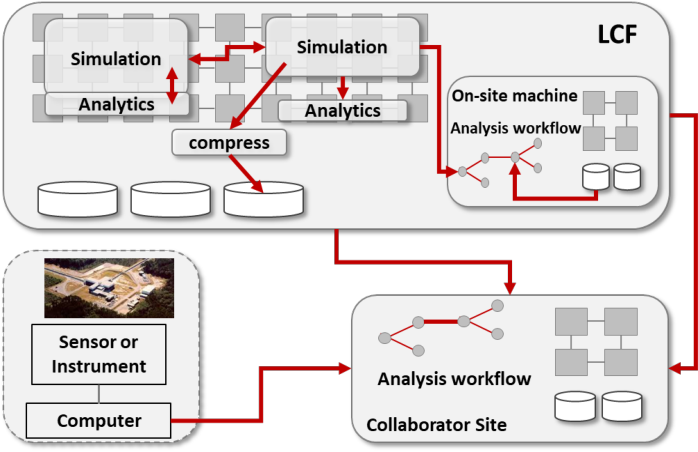
\includegraphics[scale=.75]{figures/ExampleWorkflow.pdf}
\caption{Example workflow using ADIOS in a number of ways. NEEDS to be edited..}
\label{fig:example_workflow}
\end{figure}

The number of engines available in ADIOS provides a large amount of flexibility when selecting a configuration. Further, multiple executables can be connected using the read/write API of an ADIOS engine to support a range of different types of workflows. The example workflow in Figure~\ref{fig:example_workflow} shows a simulation using ADIOS engines to transfer data in a number of different ways. \todo{Dave: Finish this....}

There are a number of factors to consider when deciding which ADIOS engine to use. First and foremost, the choice of engine may depend on a future use case for the data, such as post hoc analysis. In this case, the engine can save data using either the BPFile or HDF5 file formats. For other cases, a number of factors should be considered when choosing the most appropriate engine.

One method to aid in choosing the most appropriate engine for a given scenario is by using a set of empirical and speculative comparison factors~\cite{Kress-isav15}. These comparison factors allow the three classes of engines (file based, in-line based, and in-transit based) to be classified and evaluated. \todo{talk about fault tolerance} Below we list six of the most relevant these comparison factors, and explore the strengths and weaknesses of the different classes of ADIOS engines in relation to those factors. By understanding the strengths and weaknesses of each engine type, it will be possible to make an informed choice of engine selection based the needs of a given use case.

\paragraph{\emph{Data Access:}}
Data access is defined as the ability to access the full breadth of a simulations data, and is also concerned with both the temporal fidelity and temporal range of available data.
\begin{itemize}
    \item \emph{File based methods} generally do not have great data access in terms of data breadth and temporal fidelity. That is, it is generally too expensive to save out all of a simulations state, so data are first culled before being written to disk, while also often skipping many time steps between writes. However, these methods do have the best temporal range, as it is trivial to scan forward or backward in time in a file.
    
    \item \emph{In-line methods} have very good data access. Since the visualization is running on the same node where the data are being generated, they generally have access to all of the simulations data. This also means that they have good temporal fidelity, as they can conceptually operate on every simulation time step. However, in-line methods generally have poor temporal range. This is because once a time step has passed, the visualization routine would have to store it in memory in order to access it later. That said, the available temporal range can be modified by the user depending on how much memory they are willing to devote to storing past time steps. 
    
    \item \emph{In-transit methods} can have very good data access. This access however, depends on how much data a user is willing to send across the network to the in-transit methods. Generally, this is not everything that the simulation produces, so visualization routines may be more limited in this setting. Temporal fidelity can also be very good with in-transit, as every step can be gathered from the simulation if needed. However, these methods suffer the same temporal range issues as in-line methods, where range is user and system dependent.
\end{itemize}
\textbf{Table sub categories:} spatial access, temporal access, temporal range
\begin{itemize}
    \item File: - - +
    \item Inline: + + -
    \item Intransit: 0 0 0 (???)
\end{itemize}

\paragraph{\emph{Data Movement:}}
Data movement is defined as the amount of data being sent from a simulation process. That data can either be sent to disk, to another node in the simulations allocation, or a separate allocation entirely. 
\begin{itemize}
    \item \emph{File based methods} suffer the most in terms of data movement. Writing data to disk is a slow operation, and writing large amounts of data can stall a simulation for large periods of time. 
    
    \item \emph{In-line methods} data movement can can range from none, to simulation stalling levels. This is because some visualization algorithms traditionally require large amounts of inter-node communication which can be enormously expensive compared to a smaller node allocation. \todo{does this go in scalability?}
    
    \item \emph{In-transit methods} have a different issue with regards to data movement. Before visualization can take place, the data must be sent from the simulation to a visualization resource for processing. This dump from the simulation to the visualization resource has the potential to cause network interference or even slowdown the simulation while data is sent. However, this data transmission has potential to end up moving far less data, in total, than in-line visualization. This is due to the amount of inter-node communication that takes place during communication heavy visualization routines, meaning that in-transit will have to send less data since they typically operate on smaller allocations.
\end{itemize}
\textbf{Table sub categories:} None
\begin{itemize}
    \item File: -
    \item Inline: +
    \item Intransit: 0
\end{itemize}

\paragraph{\emph{Scalability:}}
Scalability is defined as the ability of a visualization and analysis task to efficiently utilize the resources it is given.
\begin{itemize}
    \item \emph{File based methods} 
    
    \item \emph{In-line methods} are constrained to running on the full allocation of the simulation. While this level of concurrency can be advantageous for embarrassingly parallel algorithms that perform little synchronization or communication, it can be a bottleneck for routines that require significant communication (e.g. particle advection), or algorithms that don't scale up to the levels of simulation codes (e.g. hundreds of thousands of cores).
    
    \item \emph{In-transit methods} have the benefit that the visualization resource can be appropriately configured for the tasks to be performed.  Algorithms that require significant synchronization and communication will generally perform much better at lower levels of concurrency, and this can be used to optimize the performance.
\end{itemize}
\textbf{Table sub categories:} I/O, compute-heavy, comm-heavy
\begin{itemize}
    \item File: - 0 0
    \item Inline: + + -
    \item Intransit: 0 + +
\end{itemize}

\paragraph{\emph{Coordination:}}
Coordination is defined as the need for a visualization and analysis task to coordinate with the state of the simulation. This factor is concerned with such items as ensuring data is moved and available for use, how to handle missing or incomplete data, and what to do if visualization resources are not available. 
\begin{itemize}
    \item \emph{File based methods} require no coordination.
    
    \item \emph{In-line methods} require minimal coordination. If visualization code is embedded in the simulation, coordination is as the visualization routine at the end of the simulation main loop. For production tools like LibSim and Catalyst the coordination is very similar, but the call is made into the particular library.
    
    \item \emph{In-transit methods} require much more coordination. At every simulation cycle where visualization needs to be performed calls must be made to transfer the data to the visualization resource. This transfer requires use of the network and coordination on both the sending and receiving side to ensure the data are successfully sent and received. This method also has a particular pitfall in that the visualization resource may not available for some reason to receive data, meaning the sender has to have rules about how to proceed in this case.
\end{itemize}

\textbf{Table sub categories:} None?
\begin{itemize}
    \item File: +
    \item Inline: +
    \item Intransit: -
\end{itemize}

\paragraph{\emph{Resource Requirements:}}
Resource Requirements is defined as the additional resources that a visualization and analysis task needs in order to execute.
\begin{itemize}
    \item \emph{File based methods} use the simulations resources to write the data to disk, so no extra resources are required to save the data. These methods do however require extra resources when the data is analyzed after the simulation is complete. The amount of resources need to do this analysis can vary depending on the required task. 
    
    \item \emph{In-line methods} share the simulation resources with the visualization routines. This coexistence can have negative implications for the simulation of the visualization routines require large amounts of memory or communication, which can add to the simulations cost. Therefore simulations will generally dedicate a fixed window of time for visualization, while placing restrictions on memory or even network use.
    
    \item \emph{In-transit methods} by definition require additional resources, adding those resources as extra cost to a running simulation. However, these additional resources can be used asynchronously once the data are transferred, allowing the simulation to proceed after transmitting data. Special care must be taken to allocate the right amount of resources for the visualization task at hand, or the resources might not be ready the next time the simulation is ready to send data.
\end{itemize}

\textbf{Table sub categories:} Use sim resources, use extra resources
\begin{itemize}
    \item File: 0 -
    \item Inline: - +
    \item Intransit: 0 -
\end{itemize}

\paragraph{\emph{Exploratory Visualization:}}
Exploratory Visualization is defined as the ability to visually sift through data coming from the simulation in order to find features of interest.
\begin{itemize}
    \item \emph{File based methods} can have access to the full spatio-temporal data from the simulation, but generally only have access to subsets of data, or very sparse temporal data. File based methods though have the benefit of not blocking the simulation, and the data can be explored and visualized for as long as needed.

    \item \emph{In-line methods} have access to the full range of spatio-temporal data from the simulation. The downside of this method for exploratory visualization is that the exploration will come at the cost of pausing the simulation while a time step is explored interactively.
    
    \item \emph{In-transit methods} can have access to the full spatio-temporal range of the simulation, but are generally more restricted, and only receive a subset of the full simulation state. However, this method has the benefit of being able to perform exploratory visualization while not blocking the simulation, since the simulation can proceed asynchronously while a given time step is explored.
\end{itemize}
\textbf{Table sub categories:} spatio-temporal access, block simulation
\begin{itemize}
    \item File: + + (?)
    \item Inline: + -
    \item Intransit: 0 +
\end{itemize}

\paragraph{\emph{Fault Tolerance:}}
Fault Tolerance is defined as a methods resilience to causing an irrecoverable problem for the simulation, causing it to crash. 

\begin{itemize}
    \item \emph{File based methods} are very resilient to faults.
    
    \item \emph{In-line methods} can have significant issues with fault tolerance. This is because the visualization and simulation run together on the same resource, and the visualization can expose the simulation to data corruption, infinite loops, or errors from visualization routines.
    
    \item \emph{In-transit methods} are inherently more fault tolerant because of the clear and distinct separation between the simulation and the visualization resources and binaries. In this paradigm the data transfer to the visualization resource becomes the main point of exposure to faults.
\end{itemize}
\textbf{Table sub categories:} None
\begin{itemize}
    \item File: +
    \item Inline: -
    \item Intransit: +
\end{itemize}


\begin{table}
\centering
\caption{Table caption}
\label{table:comparisonFactors}
\renewcommand{\arraystretch}{1.5}
\setlength{\tabcolsep}{8pt}
\begin{tabular}{
>{\columncolor[HTML]{EFEFEF}}c |ccc}
\hline
\multicolumn{1}{l|}{\cellcolor[HTML]{EFEFEF}} & \multicolumn{3}{c}{\cellcolor[HTML]{EFEFEF}\textbf{Method Type}} \\
\textbf{Comparison Factor} & \multicolumn{1}{l}{\cellcolor[HTML]{EFEFEF}\textbf{File}} & \multicolumn{1}{l}{\cellcolor[HTML]{EFEFEF}\textbf{In-line}} & \multicolumn{1}{l}{\cellcolor[HTML]{EFEFEF}\textbf{In-transit}} \\ \hline
\begin{tabular}[c]{@{}c@{}}\textbf{Data Access}\\\emph{(Spatial Access, Temporal Fidelity, Temporal Range)}\end{tabular} & - - + & + + - & 0 0 0 \\
\textbf{Data Movement} & - & + & 0 \\
\begin{tabular}[c]{@{}c@{}}\textbf{Scalability}\\\emph{(I/O, Compute-heavy, Communication-heavy)}\end{tabular} & - 0 0 & + + - & 0 + + \\
\textbf{Coordination} & + & + & - \\
\begin{tabular}[c]{@{}c@{}}\textbf{Resource Requirements}\\\emph{(Uses Sim Res., Uses Extra Res.)}\end{tabular} & 0 - & - + & 0 - \\
\begin{tabular}[c]{@{}c@{}}\textbf{Exploratory Visualization}\\\emph{(Spatio-temporal Access, Block Sim.)}\end{tabular} & + + & + - & 0 + \\
\textbf{Fault Tolerance} & + & - & + \\ \hline
\end{tabular}
\end{table}







\subsection{Operators}
ADIOS supports operators as a mechanism for performing calculations on the data before it is written by the engine.
A general purpose operator, called a Callback provides the user with the ability to perform arbitrary calculations and manipulations to the data inside the engine.
Data compression is also implemented as an operator, and provides the ability perform lossless and lossy compression using a variety of techniques.
Details of the compression operators are described below.


\subsubsection{Compression}



\subsection{ADIOS Ecosystem}
The flexibility of the data movement abstractions provided by ADIOS makes it easy to integrate into other tools. The ``file-like'' API provided by ADIOS allows seamless reads from disk, from memory, or streaming over the network. Likewise, on the write side, the data can be sent to disk, memory or streamed across the network.
Below we discuss several tools that make use of the the ADIOS API for data related tasks.

\subsubsection{Visualization Tools}
The visualization tools VisIt~\cite{HPV:VisIt} and ParaView~\cite{paraview} both support reading data from ADIOS.
Both tools provide access to ADIOS data using a data reader plugin.
The plugin reads the ADIOS data and creates mesh-based data that can be visualized by the VisIt and ParaView tools.
Using the ADIOS API, both tools access data coming from any ADIOS engine, including files or streaming.
An example of VisIt visualizing streaming data is described in Section~\ref{sec:jaxa}.



\subsection{Code example}

\section{Example Use Cases}
\label{sec:examples}

In this section we demonstrate how the I/O abstraction and engines described above in Section~\ref{sec:adios} can be used with different applications. These examples show how ADIOS engines can be used in different ways to accomplish the in situ processing required by a scientific campaign. The examples show how in situ can be used in both shared and separate resource configurations, and also include an example where data was streamed across the wide area network (WAN). In each example, we motivate the purpose of each scientific example and how ADIOS was used to provide the solution.

\begin{comment}
\subsection{Simple inline visualization: Owner Jong}
\todo[inline]{Majority of text from James' paper: Binning Based Data Reduction for Vector Field Data of a Particle-In-Cell Fusion Simulation.}
Visualization algorithms are particularly sensitive to I/O bandwidth, causing the community to turn to in situ techniques to alleviate this growing problem. There has been significant work and success with the in situ visualization paradigm. One of our motivating applications is XGC1, a plasma fusion simulation code that runs at scale on supercomputers. XGC1 is a gyrokinetic particle-in-cell code that is used for modeling the physics of plasmas in fusion tokamak devices. XGC1 uses a large number of particles to represent the kinetic behavior of the plasma.
Among the data sets XGC1 generating, fusion scientists are interested in looking at particle data coming from the simulation at a finer temporal fidelity than is currently possible in a post-hoc processing. In the post processing, particle data is only saved out at each of the simulation checkpoints, which only occur between every 100 and 1,000 time steps, leaving a large temporal gap. 
 
To overcome this issue of the large temporal gap, we have created a workflow for the in situ application of a data binning technique to the particle data from the simulation~\cite{kress2019binning}. The binning technique generates vectors in each of the bins that represents the speed and direction of particles within that cell’s region. Furthermore, this technique allows the scientists to tune the binning code for both specific accuracy and speed requirements by modifying the size of the binning grid, and the number of particles used to extract the vector field.

With this simple yet flexible subsampling method, we have  provided significant data reduction and in situ visualization performance so that scientists can have online particle movement information during runtime.
\end{comment}

\subsection{Strong Coupling in a Fusion Simulation}

%There are four engines in ADIOS that support strong coupling: the Sustainable Staging Transport (SST) engine, the Strong Staging Coupler (SSC) engine, the Insitu-MPI engine, and the BP4 engine. 
%The SST engine is designed to be a general-purpose staging engine that supports highly flexible configurations. Users can choose from several different underlying data transport methods, including RDMA, TCP, UDP, and shared-memory. The buffering mechanism in SST also provides several options to address different application requirements. 
%It can be configured to buffer a certain number of data steps, and when the buffer is full, it can block the writer processes, or it can delete old steps and ensure there is always space for writing newer steps. In strong coupling use cases, this buffer limit usually needs to be set to 1, thus every step is assured to be read by the readers before the application moves onto the next data step. The SST writer engine aggregates metadata for every single step, and shares it with all readers. Readers then issue remote reading operations based on the I/O pattern in metadata. Thus, it allows the I/O pattern to vary over time. SST also allows readers to disconnect and reconnect while writers keep writing. 
%While SST aims to provide the flexibility for addressing various application requirements, the fact that it does heavy metadata management work for every single step may become an overkill for use cases where metadata does not change frequently over time. For use cases where the metadata is constant across the workflow, a single aggregation operation will suffice.
%%The Insitu-MPI engine is motivated by this idea, and it is designed to only aggregate metadata once at the first data step. After that, every writer and reader knows the exact I/O pattern, and thus writers can directly send data to readers that request it using MPI send and receive through the world communicator. This requires the writer application and the reader applicaiton to be launched within a single mpiexec command in the MPMD mode. For extremely large applications that have constant I/O patterns, the Insitu-MPI engine can save a considerable amount of CPU time on metadata management, compared to the SST engine. However, the fact that it is based on the MPI MPMD mode makes it unfeasible to allow any writer or reader to join or quit dynamically at runtime. 
%
%The SSC engine is also designed for applications that have constant metadata over time. Similar to the Insitu-MPI engine, the SSC engine only aggregates metadata once at the very first step. Instead of using MPI send and receive functions in the Insitu-MPI engine, the SSC engine uses one-sided MPI communications. The one sided MPI paradigm does not require the writer and the reader to call send and receive functions in pairs, and instead, it allows a writer or reader to directly access the remote memory of another reader or writer. Thus, in very large scale coupling use cases, it saves overheads of one side waiting for the other side to complete the send and receive pair. 

%Most coupling uses cases require an N-to-M communication pattern where N and M are much smaller than the total number of staging readers and writers. Nevertheless, there is still use cases that require very large scale all-to-all communications, and for these applications, network based staging methods may not be optimal any more. Taking this into account, we developed the staging-over-file method in the BP4 engine, which allows applications to read a BP4 data set while it is being written. The advantage of the staging-over-file method over all other network based staging methods is that it needs less globally blocking function calls for sharing metadata and synchronizing step completion information. These globally blocking function calls can be very expensive in large scale all-to-all communications, and when this cost goes greater than the filesystem overhead, the staging-over-file method then outperforms the network based staging methods. 

High-Fidelity Whole Device Modeling (WDM) of Magnetically Confined Fusion Plasmas is among the most computationally demanding and scientifically challenging simulation projects.
The ten-year goal is to have a complete and comprehensive application 
that will include all the important physics components required to 
simulate a full toroidal discharge in a tokamak fusion reactor. 
The main driver is based on the strong coupling of two advanced and 
highly scalable gyrokinetic codes, XGC and GENE, where the former is a 
particle-in-cell code optimized for the treating the edge plasma while 
the other is a continuum code optimized for the core.
Applications for additional physics are intended 
to be coupled in the future, e.g. ones for material wall interactions or
for high energy particles.

In the WDM workflow, the ADIOS BPFile engine is used to save checkpoint/restart files, 
offloads variables for in situ analysis and
visualization~\cite{escience2018}. 
For in-memory data exchange, the SST and Insitu-MPI engines are used for coupling of the core and edge simulations~\cite{dominski2018}.
To date, three-dimensional field information has been
shared between XGC and GENE, but a five-dimensional distribution 
function-based coupling is now under development. Published results~\cite{escience2018, dominski2018}
have all relied on synchronous exchange, but asynchronicity will need to
be explored in order to mitigate blocking while data are not available. The ADIOS SSC engine is designed to support the asynchronous WDM coupling workflow. 
ADIOS affords both performant scalability as data sizes grow with 
increased dimensionality, as well as APIs that support asynchronous
operation.
% The synchronous exchange has been done using the Insitu-MPI and SSC ADIOS engines.
% Asyncronous coupling is being explored using the SST ADIOS engine.

\subsection{Streaming Experimental Data}

Fusion experiments provide critical information to validate and refine simulations that model complex physical processes in the fusion reactor as well as to test and validate hypotheses. 
Recent advances in sensors and imaging systems, such as sub-microsecond data acquisition capabilities and extremely fast 2D/3D imaging, allow researchers to capture very large volumes of data at high rates for monitoring and diagnostic purposes as well as post-experiment analyses. For example, JET, the world's largest magnetic confinement plasma physics experiment in the UK, is producing about 60 GB of diagnostic data per pulse~\cite{farthing2006data}. A 2-D spatial imaging system, called Electron Cyclotron Emission Imaging (ECEI), in KSTAR, Korea, alone can capture 10 GB of image data per 10 second shot~\cite{yun2010development}.

\begin{figure}[b]
\sidecaption
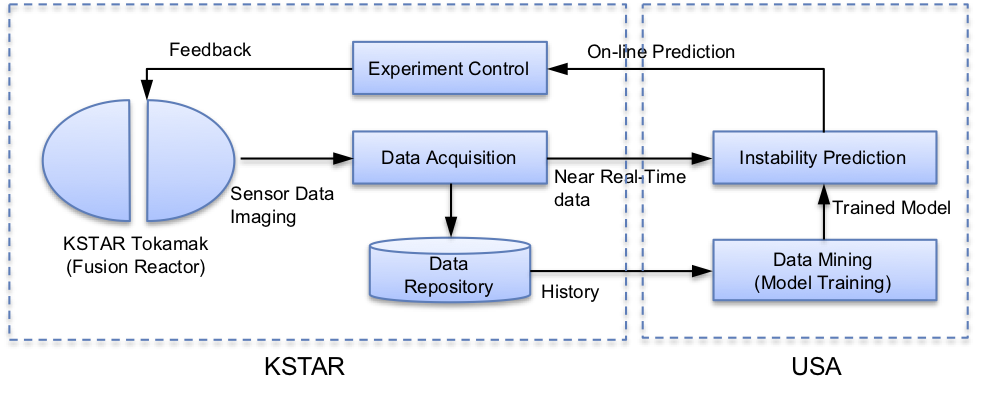
\includegraphics[width=1\linewidth]{figures/kstar-workflow.png}
\caption{Fusion instability monitoring and mitigation workflow.}
\label{fig:fusion_workflow}
\end{figure}

A system using ADIOS has been developed for KSTAR to support various data challenges by executing remote experimental data processing workflows in fusion science. It is one of the drivers for the development of the DataMan engine to support science workflows execution over the wide-area network (WAN) for near-real-time (NRT) streaming of experiment data to and from an experiment site and remote computing resource facilities. 

An example of KSTAR workflow is shown in Figure~\ref{fig:fusion_workflow}. This workflow is a multi-level workflow in that each box consists of one or more sub-workflows, each of which can be composed with ADIOS engines. One of the main goals is to stream online fusion experiment data from KSTAR in Korea to a computing facility in USA in order to perform various computational intensive analyses, such as instability prediction and disruption simulation. 
While our previous effort~\cite{choi2013icee} focused on building remote workflows with data indexing, we are currently working on composing the KSTAR workflow with DataMan. In this workflow, we use ADIOS' DataMan engine to move raw observational data as streams from Korea to the USA. Once data streams arrived in a USA computing facility, we launch a set of analysis and visualization workflows to perform denoising, segmentation, feature detection, and selection for detecting any instabilities. 
Visualization results can be delivered back to Korea for designing the next upcoming shots. 
In short, ADIOS engines enable researchers to compose and execute workflows spanning local resources and remote large-scale high performance computing facilities for NRT analysis and decision-making. 

%The volume, velocity, and variety (data elements from thousands of sensors) of KSTAR data make it extremely challenging for researchers to analyze the data only using computational resources at experiment facilities. Moreover, near-real-time (NRT) analysis and decision-making is of paramount importance in fusion experiments. 
%Researchers need ability to compose and execute workflows spanning local resources and remote large-scale high performance computing facilities.  
%Monitoring, predicting, and mitigating instabilities during an experiment need strong NRT analysis capabilities. 
%Unstable high-energy plasmas can cause serious damage to the reactor chamber, costing hundreds of millions of dollars to repair or substantial loss in productivity. 

%We have been developing an ADIOS based middleware to support various data challenges on executing experimental data processing workflows in fusion science, including development of DataMan engine in order to support science workflows execution over the wide area network (WAN) for near-real-time streaming of experiment data to and from an experiment site and remote computing resource facilities. 
%We focus on how we execute remote workflows over WAN with NRT requirement.

%An example of workflow to monitor, predict, and mitigate instabilities is shown in Figure~\ref{fig:fusion_workflow}. This workflow is a multi-level workflow in that each box consists of one or more sub-workflows. 

%To facilitate more efficient experimental work in fusion science, analysis workflows and underlying middleware infrastructure to execute them on local and remote resources should be able to handle thousands of streams of multi-dimensional sensor data within near-real time analysis constraints. 





\subsection{Interactive In Transit Visualization}
\label{sec:jaxa}
The Japan Aerospace Exploration Agency (JAXA) has implemented various ways for visualizing one of their CFD simulations, upacs-mc-LES. The visualization of CFD data consists of both batch and interactive visualization. Batch visualization is performed to create preset view images of the flowfield. Interactive visualization is conducted by interactively using Visit to understand the physics of the flowfield. While interactive visualization is not performed all the time during simulation, it is essential to have the capability to launch and attach the visualization process to the simulation when necessary, then to seamlessly detach when finished.

The agency has a heterogeneous HPC system, the Supercomputer System Generation 2 (JSS2). The main computer is a Fujitsu supercomputer with FX100 CPUs specialized for vector computations. Another cluster with x86 processors and GPUs is available for visualization and GPU-based analysis. There is a shared Lustre file system, which can be used for post-processing. An Ethernet and InfiniBand network connects the two machines, but only a portion of the nodes can communicate between the two machines. Most of the nodes can only communicate with other nodes on the internal network.

Batch visualization in post-processing is an easy way to produce movies of preset 3D visualizations on the GPU cluster, but it is stressing the file system and cannot support the largest simulations due to the I/O overhead. In situ visualization based on LibSim~\cite{libsim} is another approach, where the main computer is used to produce the images within the simulation code. In situ not only allows for producing a movie without dumping all data to disk but it also allows for interactive data exploration. ADIOS makes another approach feasible: in transit visualization where the simulation data is streamed from the main computer to another application, which in turn uses LibSim to create the visualizations. The visualization can be performed either on the main computer or on the GPU cluster (see Fig.~\ref{fig:insituJAXA_arch}). In all cases, Visit is used as the GUI for attaching to the visualization in case the user wants to interactively explore the data set.

\begin{figure}[b]
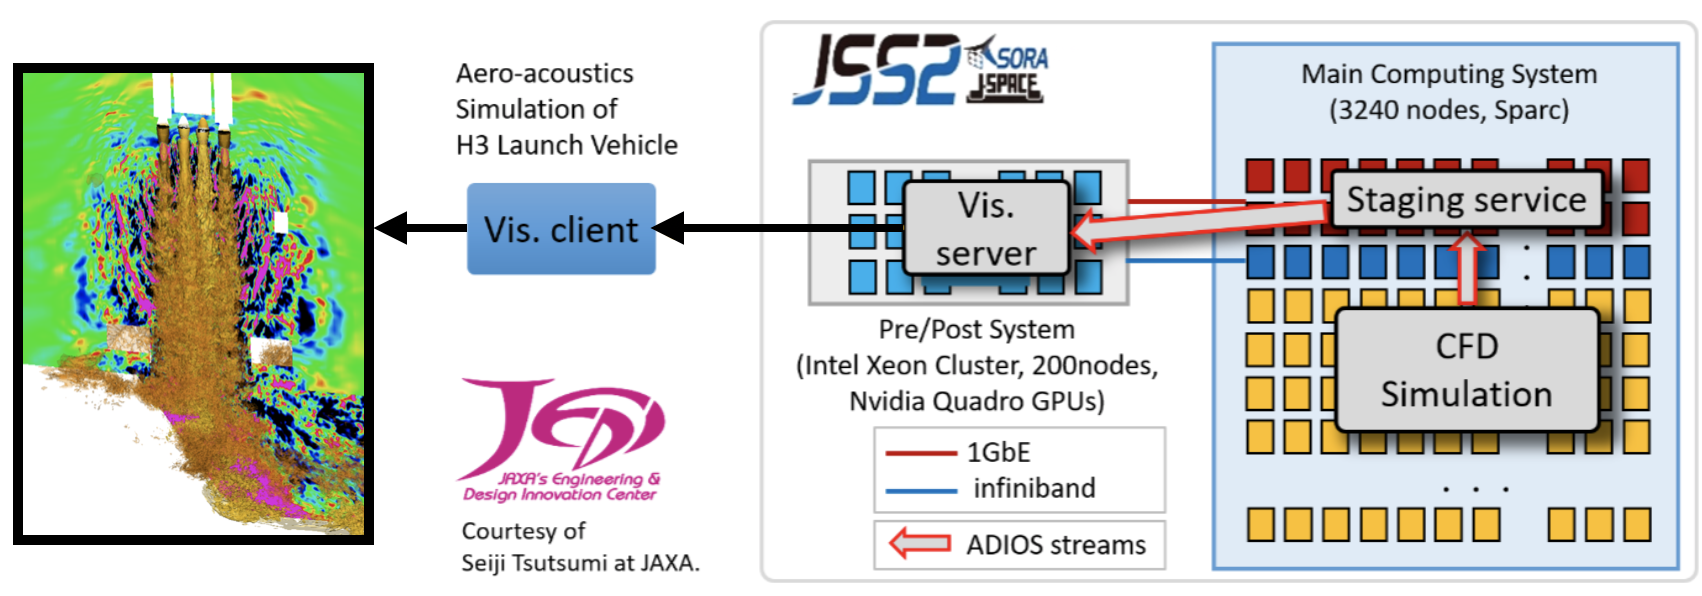
\includegraphics[width=1\linewidth]{figures/JAXA.png}
\caption{Two steps of staging of data necessary on the JAXA heterogeneous system for interactive visualization. Simulation data is staged to a concurrent staging service on nodes that have network connections to the GPU cluster. The data is further staged to the visualization server running on the GPU cluster. The visualization client then visualizes the data. The visualization on the left shows acoustic waves on the cross section and exhaust jet are visualized by normalized pressure fluctuation and iso-surface of temperature, respectively.}
\label{fig:insituJAXA_arch}
\end{figure}

The main drawback of in situ visualization with LibSim, for interactive exploration, is that the simulation process stops during interactive visualization. JAXA users want the simulation to progress with the computation while they are looking at a snapshot in time. In transit visualization using the ADIOS SST engine solves that problem and is as easy to use as in situ visualization when launching them as two separate applications together on the main computer in a single job.

Another advantage of in transit visualization (both for batch and interactive visualization) is that the simulation is not affected by the visualization process in terms of computing performance, nor by abnormal termination of the visualization process. The simulation progresses independently from the visualization and therefore the cost of visualization is amortized. On the other hand, data movement also has a cost and this offsets some of the advantages. 
As discussed in Section~\ref{sec:implications}, there are trade-offs between the in situ and in transit approaches, and it depends on the simulation size, data size and visualization cost in order to determine which approach works best. Therefore, JAXA wants to maintain and provide all approaches to visualization for its users. 

In transit visualization also provides the capability to use the GPU cluster for the visualization. The main difficulty with using a separate machine is that two jobs need to be submitted to two different machines and run at the same time.
Current job scheduling policies only support batch processing. Therefore, the only way to do interactive visualization on the GPU cluster is to submit an interactive job once the simulation is running.
This is fine for interactive visualization where the user is present. Although ADIOS makes it possible to run the visualization application immediately and let it wait for the connection to the simulation indefinitely, for a batch visualization of an overnight job, this is still a waste of resources (on the GPU cluster).

Lastly, note that using ADIOS in the simulation to output the data, the target for the data can be a concurrent application for batch visualization on the main computer, or an application on the GPU cluster for interactive/batch visualization, or it can be the Lustre file system for storing data for post-processing. The visualization application is also the same for all the three cases. It is only a matter of the runtime setup and the choice of the ADIOS Engine to run any of these cases. 

%\section{Interactive In Situ Visualization on Heterogeneous Resources}


%\section{Code Coupling}

%\section{Streaming experimental data}

%\section{Tradeoffs}
Discuss tradeoffs for the placement of visualization (in situ and in transit), and data compression....

\subsection{Placement}

\subsection{Compression}

\section{Conclusion}
\label{sec:conclusion}

ADIOS was designed from the observation that the API describing traditional I/O to the file system could be abstracted to describe more complicated data movement. 
Since applications almost always read and/or write data to storage it becomes straightforward to replace the traditional I/O mechanism with an abstraction layer that supports much more complex movement of data with minimal changes to the flow of execution.

In this chapter we have described the high level design of the ADIOS library as well as a description of the currently available engines. We also provided a comparative discussion on each engine and discussed their strengths, weaknesses, and where each is most suitable. To provide some concrete examples of how ADIOS has been used in practice, we described a number of experimental and simulation examples that use ADIOS in their workflow for in situ processing and visualization.

\section{Acknowledgements}

This research was supported by the Exascale Computing Project (17-SC-20-SC), a collaborative effort of the U.S. Department of Energy Office of Science and the National Nuclear Security Administration.

%\section{Comments from reviewers}

summary of changes needed:
\begin{itemize}
    \item Reviewer 1
    \begin{itemize}
        \item check list of simple TODOs
        \item Unify with introduction terms, etc. in situ, in line, in transit
        \item create space to address how ADIOS address the in situ challenges from the intro.
        \item images for 3.1?
    \end{itemize}
 \item Reviewer 2
    \begin{itemize}
        \item intro figure to describe how ADIOS works
        \item +/0/- of table is hard to read
        \item this is ADIOS2, not ADIOS. (web page ref is fixed).
        \item Fix listing 2 (spills over on pages)
        \item integrate with introduction
        \item integrate section 3 so it doesn't feel tacked on.
    \end{itemize}   
    
\item Reviewer 3
    \begin{itemize}
        \item provide a top-down approach
        \item intro: include a paragraph that describes the outline of hte chapter.
        \item tighten 3.3
        \item editing pass
    \end{itemize}    
    
\end{itemize}

\subsection{Editors summary}
The paper received good scores from reviewers, and was recommended for publication, after some revisions, many of which are language and grammar issues. Among the more substantial problems, the structure of the manuscript should be refactored (this can be done without requiring much new writing) to provide a better reading flow, and the connection to the introductory chapter should be strengthened to avoid conflicting terminology. As a further possibility to improve the manuscript, the authors are encouraged to increase non-expert readability by adding bits of explanation and discussion throughout the text. Finally, the legibility of the tables should be improved. Addressing these points will allow acceptance of the paper into the book.


\subsection{Review 1}
SCORE: 2 (accept) \\

Your score: 5 \\
Justification: This chapter fits into the tools part of the book.

\noindent\textbf{Accessibility} Your score: 4\\
Justification: Motivation and impact are clear. However, there are few minor jargon and grammar issues for the authors to address:

\begin{itemize}
\item Section 1 lists the application names (e.g., Specfem3d\_globe, PIConGPU), which may not be clear to the readers of this book.
\item Outline in Page 3 misses the description for Section 2.2.
\item Page 10: first line (spat, temp, range, movement) needs to be omitted.
\item \sout{Page 11: “.. data are note” -> data are not}
\item \sout{age 16: “.. and the how ADIOS” -> and how ADIOS}
\item \sout{Page 18: “..we lunch” -> we launch}
\end{itemize}

Response: Made these modifications.

\noindent\textbf{Introductory material}  Your score: 1 \\
Justification: There are some conflicting definitions with the introductory material: the intro defines in situ as “data is analyzed as it is generated”, but Section 2.3 further separates this into in situ and in transit. In addition to this, Section 2.3.3 mentions the in-line placement method which is in conflict with both the chapter itself and the introductory material.

\noindent\textbf{Impact} Your score: 5\\

Justification: This chapter summarizes one of the state-of-the-art in situ tools, ADIOS.  Overall, the chapter is well written and has a nice flow. My only remark for the authors would be allocating more space to discuss how ADIOS addresses some of the in situ related challenges as highlighted in the introductory material of the book. Some parts can be easily omitted to create a space for this. For instance, Section 2.3 can be shortened since it has some redundancy such as programmability and fault tolerance do not change depending on ADIOS/visualization perspective, hence, separate subsections for those seems redundant. Moreover, the comparison between the post hoc and in situ is given in the introductory material, and doing that here again would create another level of redundancy. Also, Listings 3 and 4 can be omitted since they are slight variations of Listings 1 and 2, which can be described in the same way that the authors described the difference between BPFile and SST!
 modes by pointing out the required modifications at the specific line number (line #1 in this case).

My final remark would be the lack of illustration regarding the use case in Section 3.1. It would be nice to have this as in other use cases in the chapter.


\subsection{Review 2} SCORE: 1 (weak accept) \\

\noindent\textbf{Accessibility} Your score: 3 \\

Justification: The text dives in quickly to the details of ADIOS engines with little preamble or context of the broader ADIOS framework. An example workflow doesn’t come until figure 1 on page 9. Having an intro figure with a breakdown of the ADIOS components to frame the subsequent presentation in section 2 would help immensely.

The +/0/- format of the tables is difficult to parse in general, and is especially difficult to make out on the Interactivity line of each, where the columns lack sufficient spacing. Consider making these two rows, as the row description text already is.

It would help to specify that this chapter deals with ADIOS-2, as the ADIOS webpage itself mentions both versions and the chapter’s use of just “ADIOS” could be confusing to readers unfamiliar with the area.

\sout{Typo: page 3- The abstraction used by ADIOS makes it easy to move data as it does something that the application is already doing. Namely, reading and writing from files.  -> The abstraction used by ADIOS makes it easy to move data as it does something that the application is already doing, namely, reading and writing from files.}

Listing 2 is broken between pages 13-14.

\noindent\textbf{Introductory material}

Your score: 2
Justification: The chapter makes no mention of the introductory chapter. This chapter could use an expanded introduction section that better sets the stage for in situ use and ties in the broader in situ considerations of the intro chapter to the specific I/O considerations handled by ADIOS.

\noindent\textbf{Impact}

Your score: 3
Justification: This chapter presents ADIOS, a significant component of the DOE exascale strategy and a flexible system for managing both file system writes and data transfers among producers and consumers for in situ and in transit analysis contexts. That said, section 2 of the paper reads more like software documentation “man page” than a narrative presentation of the system. The coding examples are helpful for anyone looking to implement ADIOS for their simulation, but there is similar content available at the ADIOS-2 documentation site (https://adios2.readthedocs.io/en/latest/index.html) . Section 3 provides helpful examples of in situ use of ADIOS, but these feel tacked on to the end rather than an integral part of the chapter. The chapter would be more successful if these motivating examples were introduced at the beginning and ADIOS examples and feature discussions were motivated by these throughout, with references to the online docs (or other ADIOS papers) for a
more complete discussion of the feature set.


\subsection{Review 3}
SCORE: 2 (accept)

Justification: ADIOS is clearly highly relevant to ISVFCS based on its long history, number of users, ECP presence, and several standout “hero” use cases described in this chapter. There is no question that it will be included in the book. The submission clearly fits the tools category.

\noindent\textbf{Accessibility}

Your score: 3
Justification: The writing needs improvement. Below are some specific suggestions.

- The presentation should be organized in a top-down, summary-to-details fashion. E.g., the abstract dives right into details, with the last sentence actually being a better opening sentence. This pattern of bottom-up instead of top-down writing pervades the chapter, with closing sentences in several sections belonging at the start of the sections. Even the level of sections, the conclusion is a better summary of the chapter than the abstract, I think. The introduction could also use a paragraph that outlines the structure of the rest of the chapter.
- Various terms and acronyms need to be defined before they are used. Readers not from the DOE community do not know the names of codes or machines, e.g.
- Tables 1 and 2 appear in the programmability subsections, but they apply to the parent section instead.
- Various typos, grammar, and capitalization errors exist, which will require a detailed editing pass.
- I find the style of the writing not quite polished. Some of the sentences are too short, simplistic, and lack variety. Some other sections (3.3) are long and rambling and should be tightened. Some words and phrases are too casual and not scientific or specific enough (e.g., “a couple of general guidelines…”). The current state of the chapter  is acceptable for a first draft, but ought to be improved before publication.

\noindent\textbf{Introductory material}

Your score: 3
Justification: The terminology in this chapter is inconsistent with the terminology of the introductory chapter: ADIOS uses “in situ” and “in transit” rather than time and space division. This contradicts the meaning of in situ in the book, which encompasses in transit. The editors will need to decide what is the best strategy here. I suggest that it’s ok for ADIOS to continue to use their terminology consistent with their other publications, but explain the mapping between their terms and the introduction’s, before using their own. Also, in some places they mix “in situ” with “inline,” and they also mention hybrids but do not elaborate. At a minimum, they should be self-consistent in their terminology. Also, Section 2.3 presents general tradeoffs between in situ and in transit (i.e., time and space division) that are not specific to ADIOS and feel like they belong in the introductory material.

\noindent\textbf{Impact}

Your score: 5
Justification: The chapter is a summary of previous work. The impact is that the chapter provides a single source for a high-level overview of the system as well as numerous references where readers can find more details. The description of the various engines, schemas, and use cases is informative and beneficial.



\bibliographystyle{abbrv}
\bibliography{refs}
\end{document}